% \documentclass[acmtog]{acmart}
%\documentclass[acmtog,anonymous,timestamp,review,draft]{acmart}

% SIGGRAPH Asia May 2020
\documentclass[acmtog]{acmart} 
% \documentclass[acmtog,anonymous,review]{acmart} 
\acmSubmissionID{316}

% SIGGRAPH Jan 2020
% \documentclass[acmtog,anonymous,timestamp,review]{acmart}
%\acmSubmissionID{110}


\usepackage{booktabs} % For formal tables



% TOG prefers author-name bib system with square brackets
\citestyle{acmauthoryear}
\setcitestyle{square,nosort}
%\setcitestyle{nosort,square} % nosort to allow for manual chronological ordering


% \usepackage[ruled]{algorithm2e} % For algorithms
% \renewcommand{\algorithmcfname}{ALGORITHM}
% \SetAlFnt{\small}
% \SetAlCapFnt{\small}
% \SetAlCapNameFnt{\small}
% \SetAlCapHSkip{0pt}


% Metadata Information
\acmJournal{TOG} 
\acmArticle{200} 
\acmYear{2020}
\acmVolume{39}
\acmNumber{6}
\acmMonth{12} 
% DOI
\acmDOI{10.1145/3414685.3417835}

% Copyright
\setcopyright{rightsretained} 



% !TEX root =  ApproximatingDOGs.tex

\usepackage{amsmath}
\let\Bbbk\relax
\usepackage{amssymb}
\usepackage{amsfonts}
\usepackage{enumitem}
\setlist[description]{leftmargin=12pt}
\usepackage[mathscr]{eucal}
% \usepackage[ruled,vlined]{algorithm2e}
\usepackage{algorithmic}
\usepackage{microtype}
\usepackage{units}
% \usepackage{booktabs} % For formal tables
% \usepackage{color}


% compact bullet lists and enumeration environments
\newenvironment{tight_enumerate}{
\begin{enumerate}[topsep=4pt,itemindent=\parindent]
  \setlength{\itemsep}{1pt}
  \setlength{\parskip}{0pt}
  \setlength{\parsep}{0pt}
}{\end{enumerate}}

%\newenvironment{tight_itemize}{
%\begin{itemize}[topsep=4pt]
%  \setlength{\itemsep}{1pt}
%  \setlength{\parskip}{0pt}
%  \setlength{\parsep}{0pt}
%}{\end{itemize}}

\usepackage[ruled]{algorithm2e} % For algorithms
\renewcommand{\algorithmcfname}{ALGORITHM}
\SetAlFnt{\small}
\SetAlCapFnt{\small}
\SetAlCapNameFnt{\small}
\SetAlCapHSkip{0pt}


\usepackage{dsfont}
\usepackage{graphicx,wrapfig}

\usepackage{mdframed}
\mdfsetup{skipabove=\topskip,skipbelow=\topskip}
\newmdenv[	linewidth=0.75pt,
			leftline=false,
			rightline=false,
   		innerleftmargin=0pt,
			innerrightmargin=0pt]{topbot}

%\usepackage[mathcal]{euscript}

%\usepackage{amsthm}
%\newtheorem{theorem}{Theorem}[section]
%\newtheorem{lemma}[theorem]{Lemma}
%\newtheorem{proposition}[theorem]{Proposition}
%\newtheorem{corollary}{Corollary}
\newtheorem{mydefinition}{Definition}

\newcommand{\MiR}[1]{#1} % Michael
% \newcommand{\MiR}[1]{{\bf\textcolor{cyan}{MR: #1}}} % Michael
\newcommand{\OSH}[1]{#1} % Olga
% \newcommand{\OSH}[1]{{\bf\textcolor{magenta}{OSH: #1}}} % Olga
\newcommand{\osh}[1]{#1} % Olga replaced text
% \newcommand{\osh}[1]{{\textcolor{magenta}{#1}}} % Olga replaced text
\newcommand{\AI}[1]{#1} % alex
% \newcommand{\AI}[1]{{\bf\textcolor{purple}{AI: #1}}} % alex
\newcommand{\Rev}[1]{#1} % Revision
% \newcommand{\Rev}[1]{{\textcolor{blue}{#1}}} % Revision
\newcommand{\CommentRev}[1]{{\it\textcolor{orange}{#1}}} % Revision

\newcommand{\todo}[1]{{\bf\textcolor{red}{}}}%{#1}}}
\newcommand{\tododone}[1]{{\textcolor{gray!40}{}}}%{#1}}}

% % for placeholder images 
\newcommand*{\addImage}[1]{
  \vspace{20pt}
  \begin{center} [IMAGE: #1] \end{center}
  \vspace{20pt}
}
% \newcommand*{\TODOImage}[1]{\colorbox{gray!60}{\color{white}\parbox{.98\linewidth}{\vspace{20pt} #1 \vspace{20pt}}}}


%\newcommand{\newt}[1]{{\textcolor{blue}{#1}}}
\newcommand{\newt}[1]{{#1}}


%Abbreviations
% \newcommand{\figref}[1]{Fig.\ \ref{#1}}
% \newcommand{\secref}[1]{Section\ \ref{#1}}
\newcommand{\figref}[1]{Fig.~\ref{#1}}
\newcommand{\secref}[1]{Section~\ref{#1}}
\newcommand{\appref}[1]{Appendix \ref{#1}}
\newcommand{\equref}[1]{Eq.\ \eqref{#1}}
\newcommand{\defref}[1]{Def.\ \ref{#1}}
\newcommand{\lemmaref}[1]{Lemma \ref{#1}}
\newcommand{\theoremref}[1]{Theorem \ref{#1}}
\newcommand{\corollaryref}[1]{Cor.\ \ref{#1}}


% operators
\DeclareMathOperator*{\argmin}{arg\,min}
\DeclareMathOperator*{\argmax}{arg\,max}
\DeclareMathOperator*{\Proj}{Proj}


% Olga SH notation
\newcommand{\set}[1]{\mathcal{#1}}
% Transpose symbol
\newcommand{\transposeSign}{\textsf{T}}
\newcommand{\tr}{\transposeSign}


\newcommand{\R}{\mathds{R}}
\newcommand{\Z}{\mathds{Z}}
\DeclareMathOperator{\atantwo}{atan2}

\newcommand{\x}{x}
\newcommand{\p}{p}

\newcommand{\Fbo}{F_{\bar{1}}}
\newcommand{\Fbt}{F_{\bar{2}}}

\newcommand{\FAll}{\mathbf{F}}
\newcommand{\II}{I\!I}
\newcommand{\Atotal}{\mathcal{A}}



% commands specific to this paper
\newcommand{\target}{\mathcal{S}_t}
\newcommand{\result}{\mathcal{S}_d}
\newcommand{\Kmax}{\abs{K}_\text{max}}
\newcommand{\Kmean}{K_\text{mean}}
\newcommand{\E}[1]{\cdot 10^{#1}}

%\renewcommand{\ra}{\rightarrow}
\newcommand{\norm}[1]{\left\Vert#1\right\Vert}
\newcommand{\Norm}[1]{\lvert \! \lvert \! \lvert #1 \rvert \! \rvert \! \rvert}
\newcommand{\abs}[1]{\left\vert#1\right\vert}
\newcommand{\babs}[1]{\Big \vert#1 \Big \vert}
\newcommand{\bra}[1]{\left\{#1\right\}}
\newcommand{\parr}[1]{\left (#1\right )}
\newcommand{\brac}[1]{\left [#1\right ]}
\newcommand{\ip}[1]{\left \langle #1 \right \rangle }
\newcommand{\eps}{\varepsilon}


\newcommand{\alter}[1]{\textcolor{magenta}{[Alt: #1]}}
\newcommand{\opt}[1]{\textcolor{magenta}{[Opt: #1]}}
\newcommand{\rem}[1]{\textcolor{magenta}{[Rem: #1]}}

\newcommand{\LP}{\mathbb{L}}
\newcommand{\J}{\mathbf{J}}
\newcommand{\K}{\mathbf{K}}
\newcommand{\D}{\mathscr{D}}
\newcommand{\GR}{{\mathcal{G}}}
\newcommand{\I}{{\mathcal{I}}}
\newcommand{\CO}{\mathcal{C}}
\newcommand{\GI}{{\GR}_{\I}}
\newcommand{\GC}{{\GR}_{\CO}}
\newcommand{\M}{\mathcal{M}}
\newcommand{\Mevo}{{\M}_{evo}}
\newcommand{\Mgen}{{\M}_{G}}
%\newcommand{\u}{\mathscr{u}}
%\newcommand{\v}{\mathscr{v}}
\newcommand{\TD}{\ensuremath{T_{F}\D}}
\newcommand{\ND}{\ensuremath{N_{V(t)}\D}}

% Document starts
\begin{document}
% If your title is long, consider \title[short title]{full title} - "short title" will be used for running heads.
\title[Shape Approximation by Developable Wrapping]{Shape Approximation by Developable Wrapping}

% DO NOT ENTER AUTHOR INFORMATION FOR ANONYMOUS TECHNICAL PAPER SUBMISSIONS TO SIGGRAPH 2019!
% % Authors.
\author{Alexandra Ion}
\author{Michael Rabinovich}
\author{Philipp Herholz}
\author{Olga Sorkine-Hornung}
\affiliation{
  \ \ 
  \institution{ETH~Zurich}
  \department{Department of Computer Science}
  \streetaddress{Universit\"atstrasse 6}
  \city{Zurich}
  \postcode{8092}
  \country{Switzerland}}
% This command defines the author string for running heads.
\renewcommand{\shortauthors}{Ion, Rabinovich, Herholz, Sorkine-Hornung}

% A "teaser" figure, centered below the title and authors and above the body of the work.
\begin{teaserfigure}
  \centering
  \includegraphics[width=\linewidth]{figures/"figure-1_bunny_regular".pdf}
  \caption{
    Our algorithm converts a given 3D shape into a piecewise developable surface that approximates it. We wrap the model in developable patches and nonlinearly project the original mesh onto the developables. This makes our algorithm mesh-independent and allows users to choose the approximation quality. Each patch in the end result can be fabricated using sheet material, e.g., paper. 
  \label{fig:1-teaser}}
\end{teaserfigure}

% abstract
\begin{abstract}
  % !TEX root = ApproximatingDOGs.tex
We present an automatic tool to approximate curved geometries with piecewise developable surfaces. At the center of our work is an algorithm that wraps a given 3D input surface with multiple developable patches, each modeled as a discrete orthogonal geodesic net.
% We then use these patches and a nonlinear projection step to generate a surface that approximates the original input and has the same topology, but is also amendable to simple and efficient fabrication techniques thanks to being piecewise developable. 
Our algorithm features a global optimization routine for effectively finding the placement of the developable patches. After wrapping the mesh, we use these patches and a non-linear projection step to generate a surface that approximates the original input, but is also amendable to simple and efficient fabrication techniques thanks to being piecewise developable. Our algorithm allows users to steer the tradeoff between approximation power and the number of developable patches used. 
% Unlike previous works, our algorithm explicitly approximates the input surface, giving the user the ability to tradeoff between approximation power and the number of developable patches used. \OSH{I guess we need to adjust the abstract here?} 
We demonstrate the effectiveness of our approach on a range of 3D shapes. Compared to previous approaches, our results exhibit a smaller or comparable error with fewer 
%fabricable 
patches to fabricate.
% \OSH{fewer fabricable patches sounds like some of our patches are NOT fabricale. Somehow this last sentence is hard to parse...}

%To determine the location of different wrapping patches, we utilize geodesics on the input target and a graph cuts algorithm. The output of this procedure is a set of chosen geodesics on the input mesh, from which we generate target positional constraints for a a set of developable patches and followup with an additional local optimization routine. The result of our wrapping algorithm is then fed into a post-processing step, generating a surface that approximates the original input but is also amendable to simple and efficient fabrication techniques.
\end{abstract}

%CCS
\begin{CCSXML}
<ccs2012>
<concept>
<concept_id>10010147.10010371.10010396.10010397</concept_id>
<concept_desc>Computing methodologies~Mesh models</concept_desc>
<concept_significance>500</concept_significance>
</concept>
<concept>
<concept_id>10010147.10010371.10010396.10010398</concept_id>
<concept_desc>Computing methodologies~Mesh geometry models</concept_desc>
<concept_significance>500</concept_significance>
</concept>
</ccs2012>
\end{CCSXML}

\ccsdesc[500]{Computing methodologies~Mesh models}
\ccsdesc[500]{Computing methodologies~Mesh geometry models}

%keywords
\keywords{developable surfaces, discrete differential geometry, geodesic nets, shape modeling}


\maketitle

% !TEX root = ./ApproximatingDOGs.tex


% % % single column figure
% % \begin{figure}[h!]
% %     \includegraphics[width=\linewidth]{figures/...}
% %     \caption{....
% %     \label{fig:...}}
% % \end{figure}

% % % double column figure
% % \begin{figure*}[t]
% %     \includegraphics[width=\linewidth]{figures/...}
% %     \caption{...
% %     \label{fig:...}}
% % \end{figure*}


\section{Introduction}  
\label{sec:introduction}

Shapes that can be fabricated by bending or stamping sheets of material (e.g., metal) are highly relevant to the manufacturing industry, since these fabrication processes are more energy efficient than stretching materials. Such shapes are known as developable surfaces, best illustrated by a sheet of paper---at any point it can only be bent in one direction and cannot stretch or compress. Unfortunately, developable surfaces are difficult to design due to their globally constrained geometry, a fact that is likely evident to anyone trying to wrap a noncuboid-shaped gift.

In an attempt to relieve users from this difficult design problem, various research works investigate algorithms to automatically convert 3D shapes into piecewise developable representations. One approach is to deform a given shape until it becomes developable, i.e., until its Gaussian curvature vanishes \cite{wang2004achieving} and creases emerge \cite{stein_dev}. 
%
Other approaches automatically produce individual developable strips \cite{massarwi2007papercraft,mitani2004making} or patches \cite{Shatz:Papercraft:2006} that approximate the input shape and can be cut and assembled. 
Such piecewise approximation problems with individual patches are twofold: they involve (1)~\emph{locally} fitting a good developable representation and (2)~\emph{globally} finding a good placement for the individual developables. The aforementioned methods cover the shape locally with simple triangle strips (i.e., torsal developable surfaces \cite{Pottmann:Book:2001}) in a greedy manner: the placement of their developables relies on prior mesh segmentation (e.g., part-based segmentation) and subsequent decomposition into torsal patches.

In this paper, we propose a novel, fully automatic approximation algorithm that improves on both the local and the global aspects of the problem. 
Locally, we use \emph{general} developable surfaces instead of solely torsal patches, by employing discrete orthogonal geodesic nets (DOGs) \cite{Rabinovich:DogNets:2018,Rabinovich:DogShapeSpace:2018} in our algorithm. The DOG model is known to capture both extrinsic and intrinsic deformations of developable surfaces without suffering from deformation locking \cite{locking1,locking2,Tang:InteractiveDevelopables:2016}. This model eliminates the need for combinatorial partition of the developable surface into planar and torsal patches and results in a better coverage, since it allows to optimize over the entire developable shape space.
Globally, we determine where and how many DOGs to place by performing a \emph{global optimization} that is based on developables, i.e., the problem at hand, rather than on more generic mesh segmentation methods.  

We demonstrate how the results of our algorithm are at least comparable with or better than previous methods in terms of approximation error while requiring fewer patches, which eases fabrication (see \figref{fig:compare_4bunnies}). We compare our method with previous works in more detail in \secref{sec:results}. 

We detail our algorithm in \secref{sec:method} and summarize it below, as illustrated in \figref{fig:1-teaser}. 
The key to our algorithm is to wrap the input model tightly with DOGs, benefiting from their flexibility. 
% 1. Placement initialization
Finding a good initial guess of where and how many DOGs to fit is not a trivial step. We initialize the global placement by creating an overcomplete set of geodesics, shown in \figref{fig:1-teaser} (\emph{place}), from which we select a subset using a global multi-labeling graph-cut optimization. 
% 2. DOG fitting
The selected geodesics guide the placement of our DOG-fitting optimization process (\figref{fig:1-teaser} \emph{wrap}). Our DOG fitting is devised to prevent over-constraining, which we achieve by first using the geodesics alone as positional constraints and subsequently carefully adding more constraints to wrap and extend over a larger portion of the surface. Thanks to the DOGs' flexibility and our surface fitting process, we achieve a better coverage compared to torsal patches, as shown in \figref{fig:compare_error_torsal_vs_general}.
% 3) Non-linear projection
After wrapping the mesh with DOGs, we non-linearly project the parts of the input mesh onto the DOGs to obtain a valid, manifold, piecewise developable representation (\figref{fig:1-teaser} \emph{result}), which can be fabricated (\figref{fig:1-teaser} \emph{paper craft}). % optimize the developablility 


\paragraph{Contributions}

The contribution of this paper is a novel \emph{automatic} tool that approximates general curved surfaces by piecewise developable ones. Since we wrap the input mesh with developable surfaces, rather than deforming it \Rev{during the wrapping process, }our algorithm does not depend on information contained in the specific tessellation of the shape and is thus robust to the underlying meshing, \Rev{as we show in \figref{fig:mesh_robustness}.} 

Our specific contributions, illustrated in \figref{fig:benefits}, are as follows:
We contribute a method for fitting DOGs to general surfaces (\figref{fig:benefits}a).
% (a) Method for fitting DOGs to general surfaces.
First, while the flexibility of DOGs has been demonstrated in the context of editing systems with few, predefined position constraints, we contribute a robust method to apply DOGs to automatic surface approximation.
%
Secondly, our method allows for granularity control due to the global patch placement optimization (\figref{fig:benefits}b).
% \paragraph{(b) Granularity control by global patch placement optimization.} 
Users can specify their desired granularity in terms of number of patches, effectively trading approximation error for ease of assembly. Thanks to our global patch placement being based on developables, our algorithm 
\Rev{results in an} 
approximation under the given bounds. 


\begin{figure}[t]
    \includegraphics[width=\linewidth]{figures/"contributions".pdf}
    \caption{
    We contribute an approximation method that (a)~uses general developable surfaces, i.e., discrete orthogonal geodesic nets (DOGs). These can model surfaces that torsal patches cannot; in this example we show 3 cylindrically bent parts (signified by the green rulings) connected by a  planar part.
    % allow us to approximate the surface without an a priori understanding of the 
    % , to achieve a small approximation error. 
    (b)~The approximation power of our method can be steered to achieve variable granularity. Here, the bumpy shape is represented with 5 or 11 patches, consequently leading to a decrease in error, measured as the Hausdorff distance w.r.t.\ the bounding box diagonal. 
    % Since our algorithm does not deform the input mesh, (c) different tessellations of the same shape result in similar approximation results in terms of the piecewise developable shape.
    \label{fig:benefits}}
\end{figure}
% !TEX root = ./ApproximatingDOGs.tex


\section{Related work} 
\label{sec:related-work}


We give an overview of the representative literature on modeling and approximation with developable surfaces.

\paragraph{Modeling with developable surfaces}
The mathematical study of smooth developable surfaces is over two hundred years old \cite{DevHistory}. The past several decades have seen a significant body of work on \emph{freeform modeling} of developable surfaces, a task that requires determining a specific representation for them that is amenable to user control of the shape.
There are several such models for developable surfaces, each originating from different equivalent characterizations of developables and then possibly discretized. 
The representations are based, e.g., on vanishing Gaussian curvature \cite{wang2004achieving}, isometry to the plane \cite{grin_shells}, or the special parameterizations admitted solely by developable surfaces. The latter parameterizations include conjugate ruled nets \cite{conical, Bo:GeodesicControlled:2007, Solomon:Flexible:2012, Tang:InteractiveDevelopables:2016, stein_dev}, orthogonal or parallel geodesic nets \cite{Rabinovich:DogNets:2018,Wang2019geodesic}, 
\Rev{or isometric quadrangulation of a planar domain to achieve discrete-isometric mappings \cite{Jiang:QuadMapping:2020}. }
\Rev{Sell\'{a}n et al.~\shortcite{Sellan:RankMinimization:2020} focus on modeling developability of height fields and cast it as a convex rank minimization problem. }
% \Rev{
% Recently, Sell\'{a}n et al. [\citeyear{Sellan:RankMinimization:2020}] proposed a very different approach, to approximating developables surfaces. They observe that developability can be cast as a rank constraint and apply rank minimization techniques, yielding a convex problem. This approach has been investigated on height fields. 
% }
    
%
Different models have different strengths and weaknesses, and for the task at hand we choose different representations for the various stages of our algorithm. 


\paragraph{Approximating curved surfaces with developables}

% \paragraph{Deforming the shape.} 
The methods in \cite{wang2004achieving,stein_dev} iteratively deform an input shape until it becomes a discrete developable surface. The instability of the method of \cite{wang2004achieving}, which minimizes a vertex-based angle deficit objective (a measure of discrete Gaussian curvature) is noted in \cite{stein_dev,zhao2006triangular} and serves as a motivation for the more constrained, ruling-based developable model of \cite{stein_dev}. 

% \paragraph{Varying rulings.}
In \cite{stein_dev}, the rulings are essentially encoded in the mesh and adapted to reduce the number of developable patches. The geometrical mesh structure emerges in their developable flow process. Other methods that are more concerned with editing rather than approximating with developable surfaces allow ruling directions to vary freely within an a priori defined, global combinatorial mesh decomposition \cite{Solomon:Flexible:2012,Bo:GeodesicControlled:2007}. In contrast, Schreck et al. [\citeyear{Schreck:Crumpling:2015}] present an interactive system that recomputes the composition in a pre-defined fixed domain.

% \paragraph{Decomposition to strips or patches.}
Decomposing shapes into torsal developable surfaces, i.e., developable surfaces with non-vanishing mean curvature everywhere (no planar parts), is a popular approach. Mitani and Suzuki~\shortcite{mitani2004making} and Liu et al.~\shortcite{Liu:Stripification:2009} use planar quad (PQ) strips, Shatz et al.~\shortcite{Shatz:Papercraft:2006} fit circular cones, Massarwi et al.~\shortcite{massarwi2007papercraft} expand to generalized cones. Note that Shatz et al.\ allow for cone singularities (apexes), as visible in \figref{fig:compare_4bunnies}, which creates smoothness artifacts and may hinder some fabrication processes. All these methods perform the decomposition in a process that relies on a prior segmentation and a subsequent parameterization. 
The work of \cite{julius2005d} is similar in spirit but decomposes the input into quasi-developable patches as opposed to strips, and these patches are used to make shapes out of paper and fabric. 

Similar to our method, the works of \cite{chen_approx,pottmann_approx} employ developables to wrap an input surface. However, in contrast to our approach, these works do not consider the global nature of the problem and rather use a single ruled patch, essentially relying on the existence of a segmentation of the input mesh if one needs to approximate general geometries and topology.

The global placement of developable patches is nontrivial, therefore a number of previous works rely on user input for guidance. Sch\"uller et al.~\shortcite{schuller2018shape} decompose shapes into a single spiralling ribbon based on user-guided segmentation. Rose et al.~\shortcite{sheffer} interpolate arbitrary sketched boundary curves with developable surface strips. Tang et al.~\shortcite{Tang:InteractiveDevelopables:2016} demonstrate a user guided design tool to approximate input surfaces with piecewise spline developables, where users manually determine the initial location of each patch, unlike our work where this process is automated.


\paragraph{Position of this work.} 
We leverage the larger body of work on developable surfaces, as we detail in \secref{sec:method}, which yields preferable results of our novel approximation algorithm compared to prior methods. \figref{fig:compare_4bunnies} shows that our method produces lower error than the methods of Mitani and Suzuki \shortcite{mitani2004making} and Shatz et al.~\shortcite{Shatz:Papercraft:2006} \emph{and} fewer patches. In comparison to Stein et al.~\shortcite{stein_dev}, our method results in comparable error and \emph{fabricable} parts. Furthermore, our method allows for steering the number of resulting patches. We report the root mean square (RMS) error as the metric that previous works used.  

\begin{figure} [t]
    \centering
    % \noindent\includegraphics[width=\linewidth]{figures/"comparison 4 bunnies".pdf}
    \noindent\includegraphics[width=\linewidth]{figures/"comparison 4 bunnies - no Stein patch".pdf}
    \caption{
        Compared to previous methods, our algorithm produces comparable or lower error and fewer patches. \emph{Left to right: }Mitani and Suzuki \shortcite{mitani2004making}, Shatz et al.~\shortcite{Shatz:Papercraft:2006}, Stein et al.~\shortcite{stein_dev}, and our method. The root mean square (RMS) error is computed as cited in the original papers \cite{Cignoni:Metro:1998}. We generated Stein's bunny based on their pre-scripted example. 
        % \AI{try running Olga's code; if doesn't work, leave this}
        \label{fig:compare_4bunnies}}
\end{figure}
% !TEX root = ./ApproximatingDOGs.tex

%  NOTATION
% % specific to Approximating DOGs
% \newcommand{\target}{\mathcal{S}_t}
% \newcommand{\result}{\mathcal{S}_d}


\section{Method}
\label{sec:method}


Our input is a triangle mesh, which we  call the \emph{target shape} for the rest of this paper and denote by $\target = (V_t,F)$. Our output is a piecewise developable surface that approximates the target and is represented as a triangle mesh with the same connectivity, denoted by $\result = (V_d,F)$; we also output its segmentation to developable patches. Each patch can be fabricated by simply bending a thin sheet of material, and the entire shape can be built by joining the patches together (\figref{fig:1-teaser} \emph{paper craft}). 

As illustrated in \figref{fig:algorithm_overview}, our algorithm consists of two main steps: 
\begin{enumerate}
	\item Approximate the target with multiple developable patches.
	\item Non-linearly project the target shape onto the patches.
\end{enumerate}
%
At the first stage we wrap our target shape with multiple discrete developable patches that approximate different parts of the surface. This results in a set of disconnected,  intersecting developable patches (\figref{fig:algorithm_overview}b), which we denote by $D_i$. These patches  alone are not yet useful for fabrication purposes. At the second stage we compute our final output $\result$ 
by a special non-linear projection of $\target$ onto the collection of developable patches (\figref{fig:algorithm_overview}c). We describe our wrapping algorithm by first explaining how we fit a single patch to the target surface and then show how to compute the placement of multiple patches to approximate the entire target shape.


\begin{figure} [h!]
	\vspace{10pt}
	\centering
	\noindent\includegraphics[width=\linewidth]{figures/"method overview".pdf}
	\caption{
		Our algorithm receives the given target shape to approximate~(left). After wrapping it with multiple DOG patches, in this case 5~(middle), we perform a non-linear projection step, which outputs a piecewise developable mesh that approximates the input~(right). The colors indicate the Gaussian curvature $K$, with blue being negative and red positive $K$. 
\label{fig:algorithm_overview}}
\end{figure}
	

\subsection{Locally fitting a single developable patch} 
\label{sec:wrap_single_dev}

The process of partially wrapping a target surface with a developable surface necessitates a good model for deforming developable surfaces: one that can freely bend in arbitrary directions without being limited by a predetermined set of rulings. Likewise, we would like to use a model that can stretch while staying developable and is not fixed to a predefined isometric planar shape. We use the model of discrete orthogonal geodesic nets (DOGs)  \cite{Rabinovich:DogNets:2018}, as they allow for modeling of developable surfaces without rulings. A DOG is a mesh with regular quadrilateral grid connectivity, where for each vertex of valence greater than 2, all angles in the vertex star are equal.

We wrap the target locally by starting with a flat DOG sheet and minimizing a fitting objective. \figref{fig:single_patch_unstable} demonstrates that this is in itself a nontrivial task. Modeling with DOGs, or any other discrete model of developable surfaces, requires solving optimization problems with many non-linear and non-convex constraints. Constraining the positions of too many vertices of a DOG typically conflicts with its angle constraints and  results in an over-constrained problem, as there might not be a discrete developable surface passing through these points. As \figref{fig:single_patch_unstable} shows, over-constraining a DOG typically results in a failure in optimization. We therefore aim to find a stable way to wrap a given target surface.

\begin{figure}[h!]
\centering
\includegraphics[width=\linewidth]{figures/"over-constraining".pdf}
\caption{
	Optimizing a single DOG while setting positional constraints at all vertices at once is unstable and typically fails, resulting in a mesh that is crumpled and also does not satisfy the DOG constraints. 
	\Rev{The dots mark the positional constraints' target (blue) and current (red) locations. }
\label{fig:single_patch_unstable}}
\end{figure}


\subsubsection{Stable patch initialization} \label{sec:patch_initialization}

Both the theory of smooth developable surfaces and of DOGs shows that one can always constrain a curve on a planar sheet while deforming it isometrically \cite{do_carmo, Rabinovich:DogNets:2018, Rabinovich:DogShapeSpace:2018}. Moreover, if the target curve has non-zero curvature, then this constraint is maximal, in the sense that generally one cannot isometrically deform the sheet and constrain much more than the points on a single curve. Motivated by this, we use the curve-constraining flows of \cite{Rabinovich:DogShapeSpace:2018} to first locally force a coordinate curve on a DOG patch to lie on some isometric curve along the target mesh. Unlike the case of directly constraining all vertices of a DOG, this can be done in a safe and stable manner. By construction, a coordinate curve of a DOG can be seen as a geodesic on it. Instead of fitting this geodesic to an arbitrary isometric curve on the target, we fit it to a \emph{geodesic} with non-vanishing curvature on the target mesh (\figref{fig:constraining_geodesic_to_geodesic}).

By matching a geodesic on the DOG to a geodesic on the target we guarantee the following properties:
%
\begin{enumerate}
	\item Along the matched geodesics, the normals of the DOG patch align with the normals of the target surface.
	\item If the target mesh is developable and the chosen geodesic on it has non-vanishing curvature, the DOG wraps the target perfectly.
\end{enumerate}
%
\figref{fig:constraining_geodesic_to_geodesic} provides an illustration.  Both of the above properties are mesh-independent. The first property is a consequence of geodesics having non-zero curvature, while the second is shown in \cite{more_on_paper}. Geodesics with vanishing curvature do not have well defined normals, so these properties do not apply.

\begin{figure}[h!]
\centering
\noindent\includegraphics[width=\linewidth]{figures/"FIG fitting DOG cylinder-01".png}
\caption{
	To avoid over-constraining the initially flat DOG, we fit a geodesic in its center (initially a straight line) to a geodesic on the target mesh. Along the matched geodesics, the normals of the DOG align with the normals of the target surface.
	If the target is developable and the geodesic has non-vanishing curvature, the DOG patch wraps it perfectly. 
	\label{fig:constraining_geodesic_to_geodesic}}
\end{figure}


\subsubsection{Approximating the surface} 

Fitting a DOG geodesic to a specific target geodesic serves as a stable initialization. On non-developable surfaces, this initialization can often be improved, since the fitted patch still has some degrees of freedom.
One of the biggest advantages in using DOGs is the ability to model developable surfaces with planar parts and multiple torsal patches, without being bounded by a pre-determined torsal decomposition \cite{Rabinovich:DogNets:2018}. 
To leverage these advantages, we continue to optimize the DOG patch, using the following strategy.

To approximate the surface, our algorithm adds position constraints in the least squares sense in order to gently pull the initialized patch closer to the target surface. 
To do so, we start from the well approximated part, i.e., the geodesic on the center line, and iteratively include constraints by growing outwards on the DOG face neighborhood after each optimization step. As \figref{fig:single_patch_constraints_growing} illustrates, this deforms a DOG patch that initially cuts  through the target surface to be tangential to it.

\begin{figure} [h!]
\centering
\noindent\includegraphics[width=\linewidth]{figures/"FIG fitting DOG-02".png}
\caption{
	We optimize a single DOG patch further after the initial geodesic fitting, since it often still has some degrees of freedom. To do so, we iteratively add soft position constraints from the centerline geodesic outwards. This leads to a better target surface approximation compared to the initialization, where the patch was initially cutting the target surface.
	\label{fig:single_patch_constraints_growing}}
\end{figure}

The soft positional constraints $ C $ are constructed by projecting the target mesh vertices  $ V_t $ onto the DOG patch. We formulate the soft constraints as a quadratic objective 
%
$$ 
E_{\text{fit}}(\target) = 
\sum_{i \in V_t} \delta_i \left\lVert C(i) - V_t(i)\right\rVert ^2,
$$
%
where $V_t(i)$ is a vertex on $ \target $ and $C(i)$ is the closest point on the current DOG patch, expressed as a barycentric combination of DOG vertices. 
Again, to avoid over-constraining the patch, our algorithm only considers position constraints that are sufficiently close to the current patch shape.
The exclusion of outliers is performed by $\delta_i$, which is
$$
\delta_i = \begin{cases}
	1 & \text{ if }  \left\lVert  C(i) - V_t(i) \right\rVert \leq  \delta_{\text{distance}} \\ 
	  & \&  \left\langle N({C(i)}),\ N({V_t(i)}) \right\rangle \geq  \delta_{\text{normal}}\,, \\ 
%	1 & \text{ if }  C(F_i) = \{ \} \\ 
	0 & \text{ otherwise, }
\end{cases}
$$
where $N({C(i)})$ is the DOG normal at point $C(i)$ and $N({V_t(i)})$ is the normal of the target vertex $V_t(i)$. If several target vertices are projected onto the same face of the DOG patch, we pick one that fulfills the above criteria and set the $\delta_i$ of the others to zero to avoid conflicting constraints. 
% We use $\delta_{\text{distance}} = $ 1.1 of the average edge length and $\delta_{\text{normal}} = 0.7 $.


\subsubsection{Covering a larger surface}

The length of our DOG patch is governed by the length of the geodesic, however, its width is not specified. When we construct the patch, we set its width to a default value, which is half the largest dimension of the target shape.
However, the DOG patch might be able to cover a larger surface than its initial size if it is allowed to stretch (while remaining a discrete developable), as shown in \figref{fig:single_patch_stretching}. 
To achieve this, we relax the outlier threshold $ \delta_{\text{distance}}$.
Additionally, we apply an energy term that allows the DOG's edge lengths to change while maintaining regularity of the parameterization, as described below.

\begin{figure} [h!]
\centering
\noindent\includegraphics[width=\linewidth]{figures/"FIG fitting DOG-03".png}
\caption{
	To allow the patch to cover a larger surface, we relax the outlier threshold $ \delta_{\text{distance}} $. This leads to a larger set of position constraints in $ E_{\text{fit}} $.
	\label{fig:single_patch_stretching}}
\end{figure}


\subsubsection{Optimization}

Throughout the approximation, we optimize the DOG patch using equality-constrained SQP as in \cite{Rabinovich:CurvedFolds:2019}. We define the objective similar to \cite{Rabinovich:DogShapeSpace:2018} as a weighted sum of the terms
%
\begin{align*}
	\min \quad & w_{\text{H}} E_{\text{H}} + w_{\text{edge}} E_{\text{edge}} + 
				  w_{\text{fit}} E_{\text{fit}} \,,\\
	\text{s.t.} \quad &\text{DOG constraints},\\
\end{align*}
%
where $ E_{\text{H}} $ is the bending energy to keep the DOG patch smooth and $E_{\text{fit}}$ are the soft positional constraints described above. The term $ E_{\text{edge}} $  regularizes the edge lengths within the DOG patch. 
In the patch initialization and surface approximation step, we maintain isometric edges using the $ E_\text{edge} = E_{\text{iso}} $ from \cite{Rabinovich:DogShapeSpace:2018} (see Eq.(14), page 13). 
In the stretching step, we exchange the isometry objective with $ E_\text{edge} = E_{\text{uni-opp}}$, a term that allows the DOG's edge lengths to change, while keeping opposing edges of the same length to control the parametrization regularity \cite{Rabinovich:DogShapeSpace:2018} (see Eq.(15)). 
For all examples in this paper, we used fixed weights of $w_{\text{H}}=6.0$, $w_{\text{edge}}=1.0$, $w_{\text{fit}}=1.5$.


\subsection{Global approximation with multiple developables} 
\label{sec:approximate_multiple_patches}

Now that we know how to fit a patch to a given part of the target surface initialized by a geodesic, we need to find out \emph{where} on the surface we should place patches. General shapes most often are only piecewise developable and therefore require multiple patches to be fitted, unless they are already entirely developable. 
Our goal is to \emph{cover} our target surface $\target$ with developable patches $D_i$. More precisely, we aim to find a set of developable patches $D_i$ such that the Euclidean distance from each vertex of the target $\target$ to one of the $D_i$'s is smaller than some approximation threshold $\eps > 0$. 
Hence, the challenge is two-fold: we need to be able to \emph{locally} wrap an area of the target mesh with a single developable as detailed in  \secref{sec:wrap_single_dev}, while also \emph{globally} determining the areas each patch should cover.

Motivated by the previous section, we compute an estimate to this problem. We sample a large set of geodesics on the target surface and quickly  estimate approximate developable surfaces for them. We use these approximate developables to select a smaller subset that still covers the surface up to the given approximation threshold (\figref{fig:multi_patch_geodesic_initialization}). The corresponding geodesics then serve as the initialization for our DOG  patch fitting. We detail in the following how we compute this subset efficiently.

\begin{figure} [h!]
\centering
\noindent\includegraphics[width=\linewidth]{figures/"initialization pipeline".pdf}
\caption{
	To find where on the target we should fit DOG patches, we (\Rev{left})~sample a large set of geodesics, for which we (\Rev{center})~procedurally construct ruled developables. (\Rev{right})~We select a subset of these developables to globally cover the target. Their generating geodesics are the initializations for our DOG patches.
	Here, we randomly sample 20\% of the 2477 vertices, and select 4 geodesics as our initializers. 
	% \OSH{$E(l)$ looks weird in the figure, not like in the formula (line 638).}
	% \AI{fixed look of $E(l)$}
	\label{fig:multi_patch_geodesic_initialization}}
\end{figure}


\subsubsection{Sampling geodesics}

We sample a set of geodesics by randomly selecting vertices as their starting points and tracing them on the surface in a direction of our choice. We choose the maximum principal curvature direction \cite{Panozzo:PrincipalCurvature:2010}, since it leads to geodesics with higher curvature on cylindrical or conical parts compared to the minimum curvature direction. In fact, a geodesic in direction of minimum curvature on developable shapes is the ruling, i.e., has vanishing curvature and is therefore not a good candidate to initialize a DOG patch, as discussed in \secref{sec:patch_initialization}. 
Starting from a given vertex, we intersect a straight line in the max principle direction with a triangle edge. Similar to the line-of-sight algorithm for geodesics on polyhedral surfaces \cite{Balasubramanian:Geodesics:2009,polthier2006straightest}, we isometrically flatten the neighboring triangle incident on the edge. We continue our line on the neighboring triangle, maintaining the direction. 
By repeating this step, we can create geodesics of arbitrary length, which means that we need to find a meaningful stopping criterion.  

Since we only sample the geodesics as stable initializers for the DOG patches, we aim to trace geodesics that would represent \emph{smooth} developable surfaces. As such, our first criterion is to stop tracing a geodesic once its second order normal differences deviate too much. 
We detect this by an adaptive mean-shift variation, where we keep track of the normal differences of each path segment and evaluate whether a new normal difference exceeds a standard deviation of $3\sigma$, i.e., is an outlier, in which case we stop tracing.
This ensures that we do not trace geodesics past creases or other large dihedral angles. 
Secondly, we also prevent geodesics from winding around smaller features (e.g., the bunny's ears) by stopping when the angle sum of the path is $> 2 \pi$. Multiple windings do not offer any additional benefit for our DOG patches and complicate the approximation. 


\subsubsection{Finding a subset of initial geodesics on the target} 
\label{sec:graphcut}

As a next step, we choose a smaller set of geodesics to serve as the initializers for our DOG patches $D_i$. We aim to select geodesics that are well spaced across the target, such that they globally optimize for coverage by DOGs. Since this is merely an initialization, we only need a rough estimate of the DOG patches to assess the coverage quality. Therefore, we efficiently create ruled developable surfaces by passing a spline through each sampled geodesic.
\Rev{Using the analytic derivates of the spline, we compute} 
the ruled rectifying developable that interpolates the spline \cite{Bo:GeodesicControlled:2007}.
We compute the ruling direction as the Darboux vector $r = \tau T + \kappa B$ with $T$ being the unit-length tangent and $B$ the unit binormal of the spline. 
Since our splines often have inflection points, for which rulings are undefined \cite{do_carmo}, we compute the curve of regression \cite{Pottmann:Book:2001} and disregard very short rulings, as they indicate flat parts on the curve. The resulting ruled surfaces are a very simple representation and only serve the purpose of helping the selection of geodesics.

\Rev{To select a subset of geodesics that covers the target,} we utilize a multi-label graph cut algorithm \cite{Boykov:GraphCut:2001}. 
\Rev{We opt for this global optimization procedure since} 
this method has been demonstrated to be effective for similar problem definitions \cite{Herholz:HeightFields:2015}.
Let our randomly selected set of geodesics correspond to the labels $l_i$, for which we wish to find a minimizer.
Our data term $d(i, l_i)$ evaluates the distance from a vertex on the target $i \in V_t$ to the closest point on the ruled surface generated by the geodesic with label $l_i$. The smoothness term $s_e$ compares neighboring labels and penalizes the assignment of different labels. To do so, the algorithm traverses the edges $\mathcal{E}$ of the target $\target$ and compares the labels of the two edge vertices. 
Consequently, we formulate our energy as 
%
\begin{align*}
	E(l) = & \sum_{i \in V_t}{d(i, l_i)} + \sum_{e \in \mathcal{E}}{s(e)} \\
	\text{where }	\ \ 	& s(e) = \begin{cases}
							0		 & \text{ if } l(e_0) = l(e_1) \\ 
							\lambda  & \text{ otherwise. }
					\end{cases}
\end{align*}


\subsubsection{Fitting DOG patches}

The result of the graph cut algorithm gives us initial locations onto which we can place our DOG patches. We then follow the single DOG patch fitting algorithm as described in \secref{sec:wrap_single_dev}, by first fitting geodesics curves (\figref{fig:constraining_geodesic_to_geodesic}) and then further optimizing and improving our approximation.
Fitting DOGs, as they are general developable surfaces, improves the coverage compared to simple torsal patches with the \emph{same geodesics} as generator curves. We show in \figref{fig:compare_error_torsal_vs_general} how the error is distributed on the surface. We compute the error simply as the distances between the target $\target$ and the respective covering developables. 

\begin{figure} [h!]
\centering
\noindent\includegraphics[width=\linewidth]{figures/"coverage error init and dogs".pdf}
\caption{
	We confirm that fitting DOGs (right) results in a significantly better coverage than with torsal patches (left). Here, we compare patches using the same geodesics as initial positional constraints for the DOGs and as generator curves for the torsal patches. The maximum distance error is 7.5\% with torsal patches and 4.2\% with DOGs. The latter decreases to 3.7\% as we add another DOG to cover the top (not shown in image).
	\label{fig:compare_error_torsal_vs_general}}
\end{figure}



\subsubsection{Cover any remaining holes}

After our algorithm computes an approximating DOG for each geodesic, we evaluate the coverage of $ \target $. For every vertex in $V_t$, we measure the shortest distance to any patch, resulting in our approximation error $\eps$. 
\Rev{We visualize this error in \figref{fig:compare_error_torsal_vs_general}.} 
Our algorithm considers every vertex with an approximation error $ \eps_i > \eps_{\text{max}} $ to be uncovered, where $ \eps_{\text{max}} $ is a user-defined threshold. We define uncovered areas as connected components of uncovered vertices. As shown in \figref{fig:multi_patch_holes}, our algorithm approximates additional patches for uncovered areas using the same steps as before, i.e., it retrieves a geodesic and fits a DOG for each area. 

\begin{figure} [h!]
\centering
\noindent\includegraphics[width=\linewidth]{figures/"FIG fitting DOG-04".png}
\caption{
	After fitting multiple geodesics, our algorithm evaluates uncovered areas marked by red circles in this image. Here, the top of the \emph{Bumpy} model  remained uncovered. Our algorithm adds a patch to achieve good coverage of the target. 
	\label{fig:multi_patch_holes}}
\end{figure}





\subsection{Non-linear projection of the target onto the patches}

% \AI{(We would restructure Section 3.3 to combine the utility of the terms with their definition).}

Our wrapping algorithm returns a set of intersecting developables that do approximate the target, but also include extraneous parts that need to be culled. Simply cutting these areas might still leave us with small holes, multiple connected components and a resulting mesh with different topology than the target. Instead of \Rev{introducting and subsequently repairing} 
these topological defects, we take a different approach: We non-linearly project the target mesh onto the wrapping developables. 
\Rev{Because we use the original mesh and iteratively project it onto the DOGs, we generate a mesh that remains a valid manifold, and has the}
same combinatorics and topology as the target mesh, but is close to the developable patches (\figref{fig:algorithm_overview}c). 
\Rev{All our results shown in \secref{sec:results} are valid manifolds, we didn't encounter degenerate meshes as our output.}

As a first step we label each face of the target mesh $\target$ with the index of a close-by DOG patch. Such a labeling induces a decomposition of the mesh into connected components associated with DOG patches.
Direct projection, i.e. using the patch that is closest to face barycenters, does not yield satifsfactory results as intersections of DOG patches might lead to many isolated components. Therefore we employ a graph cut based approach, similar to the one described in \secref{sec:approximate_multiple_patches}, to obtain a labeling that is both smooth and associated faces to spatially close DOGs. We split the faces of $\target$ into connected components forming a disconnected mesh $\result$. As some vertices will appear in triangles of different labels, they will be duplicated. 
%
The non-linear projection step evolves this initial result $\result$ towards a piecewise developable surface. To this end we try to find vertex positions for $\result$ such that the following properties hold:
\begin{description}
	\item[DOG Projection:] each vertex should be close to its associated DOG surface.
	\item[Developability:] the angle defect for each interior vertex should be very small. We use a threshold of $5\E{-3}$ for the maximal angle defect.
	\item[Smoothness:] the surface should be smooth, exhibiting the least amount of wrinkling possible.
	\item[Seam Smoothness:] for aesthetic reasons and easier manufacturability we would like seams between developable patches to be as smooth as possible.
	\item[Connectedness:] corresponding vertices at patch boundaries should be colocated.
\end{description}
%
Each of these objectives is represented as a weighted term in the compound objective function 
\begin{equation} \label{eq:proj_step12}
	\nonumber
	E(\result) = w_\text{angle}E_\text{angle} + w_\text{proj}E_\text{proj}^k + w_\text{L} E_\text{L} +  w_\text{S} E_\text{S}  + w_\text{stitch}E_\text{stitch},
\end{equation}
%
where $E_\text{angle}$ sums the squared angle defects at inner vertices 
\Rev{normalized by vertex area} 
and $E_\text{proj}^k$ sums the squared distances of each vertex to the closest point on the DOG corresponding to its label. Over the course of the optimization 
we reproject vertices onto the DOGs, which allows them to slide over the patches; however, vertices remain always associated with the same DOG.
%
The term $E_\text{stitch}$ sums squared distances of corresponding vertices, 
\Rev{the pairing of which is determined at the labelling stage.} 
The term $E_\text{L}$ contains a bi-Laplacian energy, encouraging a piecewise smooth solution. 
%
Finally, the energy $E_\text{S}$ penalizes non-smooth seams. 
\Rev{This energy applies 1D smoothing on the seams by employing the combinatorial Laplace operator restricted to the graph of boundary vertices $\mathcal{N}_i$. Two boundary vertices, $x_i$ and $x_j$, are connected by an edge in this graph if they are connected by an edge in the original mesh $\target$.
We formulate this energy as
\begin{equation}
	\nonumber
	E_\text{S} = \sum_{i}  \Big\|\sum_{j \in \mathcal{N}_i}(x_j - x_i) \Big\|^2.
\end{equation}
}
% \OSH{Should we say who $x_i$'s are? It's the first time we use $x_i, x_j$ notation in the paper.}
%
Since the objective $E(\result)$ can be represented as a non-linear least-squares energy, we employ the Gauss-Newton algorithm to optimize it. To enforce developability, we use the quadratic penalty method \cite{nocedal2006numerical}, i.e., we increase the weight $w_\text{angle}$ over the course of the iterations.
%
It is well known that optimizing for vanishing discrete Gaussian curvature is generally unstable \cite{stein_dev,zhao2006triangular}. However, we increase the weight $w_\text{angle}$ after the optimization has already moved the vertices close to the DOGs, such that they describe a surface that is almost piecewise developable.
% !TEX root = ./ApproximatingDOGs.tex

\section{Results} 
\label{sec:results}

    % \AI{2) For the examples shown in the paper, provide a quantitative measure of developability (for the final, projected mesh). This information should communicate both the worst/average deviation from developability, as well as the spatial distribution over the surface. }

    % \AI{(may improve the illustration by highlighting, with thicker lines, the seams of the final collection of DOGs that approximate the targets. Different colors may be applied to DOGs and the target to make them more differentiable)}


\begin{figure*} 
    \centering
    \noindent\includegraphics[width=\linewidth]{figures/"results - doubly complex".pdf}
    \caption{
        Approximating complex shapes by piecewise developable surfaces results in a sensible abstraction, as showcased by (left) the bumpy cube, (center) the puppy, and (right) the face.
        (bumpy cube: 24 patches, $d_H = 1.7\%$, $ \Kmax = 2.9\E{-4} $, $ \Kmean = -1.8\E{-7} $; 
        puppy: 23 patches, $d_H = 3.3\%$, $ \Kmax = 2.6\E{-3} $, $ \Kmean = 3.0\E{-5} $; 
        face: 16 patches, $d_H = 2.2\%$, $ \Kmax = 9.6\E{-4} $, $ \Kmean = 1.2\E{-5} $)
    \label{fig:results_complex}}
\end{figure*}


We showcase the applicability of our algorithm on various examples. 
We cover a representative set of applications, including developable and doubly curved primitives as well as complex shapes.
\Rev{We indicate the developability of our results using the discrete Gaussian curvature $K$ on the \emph{inner vertices} normalized by their vertex area. For each result, we report the mean $ \Kmean $ and the absolute maximum $ \Kmax $.}
We indicate the shape similarity by the Hausdorff distance $d_H$, with respect to the length of the bounding box diagonal. 


\paragraph{Developable shapes. }

First, we show in \figref{fig:results_primitives_developable} (left) that our algorithm approximates trivial developable shapes, such as a cylinder and cone, smoothly. The cylinder is approximated using a single DOG patch. Although the patch is initially only half the height of the cylinder, the position constraints that allow for stretch enable the approximation with one patch. The cone is represented using two DOG patches, due to the geodesics construction. Yet, as evident in \figref{fig:results_primitives_developable} (right), both patches meet in a smooth manner, 
% \todo{\OSH{Render so that the seam is better visible?}} 
resulting in a very good representation.

\begin{figure} [h]
\centering
\noindent\includegraphics[width=\linewidth]{figures/"FIG results-primitives-developable".png}
\caption{
    Our algorithm creates smooth cylinders with one patch thanks to our stretching step in the patch fitting procedure (left). Our smooth cone consists of two patches (right), since we there are no geodesics on the cone that would cover it due to the nature of our geodesic construction. The seams meet smoothly.
    (cylinder: 1~patch, $d_H = 0.4\%$; %, \AI{$ \Kmax = x $, $ \Kmean = y $}; 
    cone: 2~patches, $d_H = 1.0\%$  %, {$ \Kmax = 0.00072 $, $ \Kmean = 0.00012 $}
    )
    \label{fig:results_primitives_developable}}
\end{figure}


\paragraph{Doubly curved primitives. }

Doubly curved surfaces are certainly more challenging and ambiguous to represent by developables. It is well known that no good solution exists to approximating a sphere with developable surfaces. As shown in \figref{fig:results_primitives_doublycurved} (left), the result of our algorithm is akin to a tennis ball. Our algorithm also succeeds at combinations of developable parts and doubly curved parts, as demonstrated in \figref{fig:results_primitives_doublycurved} (right). This example also showcases the benefit of our non-linear projection of the original mesh, in that the hole at the top is preserved.

\begin{figure} 
\centering
% \noindent\includegraphics[width=\linewidth]{figures/"FIG results-primitives-doublycurved".png}
\noindent\includegraphics[width=\linewidth]{figures/"results--sphere, dome".pdf}
\caption{
    We can approximate spheres (left) as well as combinations of developable and doubly curved shapes (right), here a cylinder with a hemisphere. The topology of the input, as demonstrated by the hole on top, is preserved by our non-linear projection. 
    (sphere: 9~patches, $d_H = 4.1\%$, $ \Kmax = 8.3\E{-4} $, $ \Kmean = 3.3\E{-6} $;
    dome: 6~patches, $d_H = 1.8\%$, $ \Kmax = 1.8\E{-4} $, $ \Kmean = -1.3\E{-6} $)
    % \ \ \ \ \AI{dome: make smoother seams}
    % \ \ \ \ \AI{remove geodesics from sphere}
    % \AI{beautify: show the geodesics also on the dome}
    \label{fig:results_primitives_doublycurved}}
\end{figure}


\paragraph{Complex shapes.}

We demonstrate the performance of our algorithm on more complex examples, shown in \figref{fig:results_complex}. We show the result of our algorithm for the entire bumpy cube in \figref{fig:results_complex} (left). We used one side of it to illustrate our method throughout \secref{sec:method}. The bumpy cube is not a trivial example, yet our algorithm produces a good approximation automatically. Similarly, our algorithm approximates the puppy (\figref{fig:results_complex} center) and face (\figref{fig:results_complex} right) models automatically while staying close to the target shape. 
%
Developable surfaces have applications, e.g.\ in architecture. We demonstrate an architectural shell example in \figref{fig:results_masonry}, which we also fabricated from paper.

\begin{figure}
    \centering
    \noindent\includegraphics[width=\linewidth]{figures/"results-masonry".png}
    \caption{
        This architectural shell showcases the use of developable surfaces for architectural design; we fabricated it from paper. The input shape consists of 3551 vertices and results in 7~patches, $d_H = 1.8\%$, $ \Kmax = 4.18\E{-3} $, $ \Kmean = 6.77\E{-6} $. 
        \label{fig:results_masonry}}
\end{figure}

% \begin{figure*} 
%     \centering
%     \noindent\includegraphics[width=\linewidth]{figures/"results - doubly complex".pdf}
%     \caption{
%         Approximating complex shapes by piecewise developable surfaces results in a sensible abstraction, as showcased by (left) the bumpy cube, (center) the puppy, and (right) the face.
%         (bumpy cube: 24 patches, $d_H = 1.7\%$, $ \Kmax = 2.9\E{-4} $, $ \Kmean = -1.8\E{-7} $; 
%         puppy: 23 patches, $d_H = 3.3\%$, $ \Kmax = 2.6\E{-3} $, $ \Kmean = 3.0\E{-5} $; 
%         face: 20 patches, $d_H =  18\%$, $ \Kmax = 7.3\E{-4} $, $ \Kmean = 8.2\E{-7} $)
%     \label{fig:results_complex}}
% \end{figure*}


\paragraph{Steering the approximation tradeoff. }

Our algorithm is automatic, yet the tradeoff between approximation error and number of patches can be steered by the user. The goal of any developable approximation highly depends on the task or preferences: while for flank milling a very small approximation error might be prioritized, for large-scale or assembly-intensive tasks, such as fabrication from sheet material (e.g., in architecture or ship building), a smaller number of patches might be desirable. Our algorithm allows steering this tradeoff, mainly governed by the parameter $\lambda$, which is the penalty in the smoothness term of our geodesics selection (see \secref{sec:graphcut}). Since we globally optimize the patch placement, increasing this penalty leads to fewer patches being selected, yet their distribution is still optimized. We demonstrate the effects of the $\lambda$ penalty in \figref{fig:results_lilium_lambda}. This confirms that when opting for fewer patches, our algorithm produces sensible abstractions. 
\figref{fig:results_bunny_granularity} showcases that the granularity adaption performs as expected on the complex models as well, such as the bunny. 

\Rev{
In our experiments shown in \figref{fig:compare_random_geodesics}, we confirm that the random set of geodesics, if  sufficiently large, does not affect the geodesic selection substantially. For shapes with a clear best fit, like the cone, the three different random sets lead to similar selected geodesics and developable representation. The Lilium model has no clear best developable fit, which results in different geodesics being selected. Nevertheless, the selected geodesics satisfy our objective of covering the target with the given granularity $\lambda$. 
}

\begin{figure} 
\centering
\noindent\includegraphics[width=\linewidth]{figures/"lambda 3x lilium".pdf}
\caption{
    Our algorithm allows steering the approximation tradeoff via the patch placement optimization. We show how increasing the penalty~$\lambda$ reduces the number of patches at the cost of higher error.
    \label{fig:results_lilium_lambda}}
\end{figure}

\begin{figure} 
\centering
\noindent\includegraphics[width=0.9\linewidth]{figures/"results - bunny granularity".pdf}
\caption{
    \Rev{(Top row)} We show the bunny in two different granularities. The left model has 18~patches and $d_H = 4.1\%$ with $ \Kmax = 2.5\E{-3} $ and $ \Kmean = 2.5\E{-5} $. The right result consists of 26~patches and $d_H = 2.8\% $, with $ \Kmax = 1.4\E{-3} $, and $ \Kmean = 7.2\E{-6} $. 
    \Rev{(Bottom row) The Gaussian curvature $K$ concentrates onto the resulting creases. We show the absolute Gaussian curvature $\abs{K}$ in red. }
    \label{fig:results_bunny_granularity}}
\end{figure}

\begin{figure} 
	\centering
	\noindent\includegraphics[width=0.98\linewidth]{figures/"random geodesics--cone, lilium".pdf}
	\caption{
        Each result stems form a different set of randomly sampled geodesics.
        For both examples, we randomly sampled 20\% of the target's vertices, resulting in 518 for the cone and 677 for the Lilium. We show the random geodesics in light gray and the selected geodesics in black. We used $\lambda=2000$ for the cone~(top) and $\lambda=300$ for the Lilium~(bottom). 
		\label{fig:compare_random_geodesics}}
\end{figure}




\subsection{Implementation}

We implemented our algorithm in C++ using libigl~\cite{libigl} for geometry processing capabilities and Pardiso~\cite{pardiso-6.0a, pardiso-6.0b, pardiso-6.0c} for solving our linear systems. The results are generated on a 2.5 GHz Intel Core i7-7660U CPU laptop with 16 GB RAM. 
Computation times for the aforementioned examples lie between 2 and 9 minutes. As this range already implies, the computation speed mainly depends on the chosen granularity, i.e., the number of DOG patches to be fitted. The target mesh resolution, i.e., the number of vertices, does not significantly affect the geodesics and the DOG fitting, but it does impact the non-linear projection step. 

Note that the initialization procedure is very efficient and constitutes only a small percentage of the overall timing. Tracing the geodesics and building approximate ruled developable surfaces is  fast, since we compute analytic rulings from the splines passing through the geodesics. The computation time for the geodesics selection via the multi-label graph cut algorithm depends on the chosen geodesics sample size.
Note that our prototype implementation currently does not utilize multi-threading. However, fitting the DOG patches as well as tracing the geodesics is trivially parallelizable. 




% %%%%%%%%%%%%%%%%%%%%%%%

% \subsection{Discussion}

% %%%%%%%%%%%%%%%%%%%%%%%

% \paragraph{Limitations.}

% Our method is designed to approximate arbitrary shapes. Beyond smoothly curved organic shapes, we demonstrate in \figref{fig:mechanical_cube-fandisk} that our algorithm can approximate shapes with sharp creases with little error as well. Sharp creases in the cube and fandisk examples are constructed by our algorithm due to the intersections of the fitted DOG patches. While the error is small, our method is not optimized towards preserving sharp creases, however, which is evident in the fandisk example in \figref{fig:mechanical_cube-fandisk}. For example, the left edge of the center piece is smoothed because the DOG fitted to both sides of the crease. Furthermore, the corners are also smoothed out. Since such mechanical shapes are typically easy to segment based on creases, we acknowledge that other approaches that build on prior segmentation (e.g., \cite{mitani2004making}) likely lead to more feature preserving solutions. Such segmentation can be integrated with our method at the placement finding stage in the future. 
% Our method is robust with respect to the tessellation of the target shape, as we show in \figref{fig:mesh_robustness}. However, since we use the vertices on the input mesh selectively as position constraints, \emph{extremely sparse} meshing
% leads to failure in finding geodesics or bad coverage due to few feasible position constraints.

% \begin{figure} [h]
% \centering
% \noindent\includegraphics[width=\linewidth]{figures/"sharp-creases".pdf}
% \caption{
%     Our method can approximate models with sharp creases. 
%     (Top)~the cube is approximated with 6 patches ($d_H = 1.2\%$ \AI{$d_H = x\% $, $ \Kmax = x $}), and the fandisk 
%     (bottom) with 17 patches, ($d_H = 1.7\% $).%, \AI{$ \Kmax = x $)}.
%     \label{fig:mechanical_cube-fandisk}}
% \end{figure}

% \begin{figure} [h]
% \centering
% \noindent\includegraphics[width=\linewidth]{figures/"mesh robustness".png}
% \caption{
%     Our is not limited to uniform meshing, but can approximate meshes that are valid manifolds.
%     \label{fig:mesh_robustness}}
% \end{figure}

% \AI{Show a more severely bad-quality input mesh than the one in Figure 19, that demonstrates the algorithm can fail if the input mesh is bad enough. Consider here not just bad triangles on a nice smooth surface, but also meshes that provide a bad approximation of the smooth surface normals. Comment about what kind of meshing is needed in this case.}

% \paragraph{Comparison with Stein et al.~\shortcite{stein_dev} } 

% We already compared our results with previous methods on the bunny example in \figref{fig:compare_4bunnies}. In \figref{fig:compare_stein}, we extend our comparison with Stein et al.~\shortcite{stein_dev}, as it is the most recent representative work in this area. We use their open source code and run several of our models with their method, taking care to select the best possible parameter settings for each example, such as energies and optimizer strategies. 
% Our method generally results in smoother approximations. The authors do acknowledge that their ``final design is largely guided by the input tessellation'' leaving the user to provide a suitable, curvature aligned mesh. We, on the other hand, use meshes that are common in 3D reconstruction or modeling software. In terms of fabrication, their method lends itself to flank milling, as they acknowledge in their paper. Our results consist of well-defined flattenable patches that can readily be fabricated from sheet material. 

% \begin{figure} [h]
%     \centering
%     \noindent\includegraphics[width=\linewidth]{figures/"comparison Stein".pdf}
%     \caption{
%         We compare several of our results to the method of  Stein et al.~\shortcite{stein_dev}, as the most recent representative of this line of work. 
%         % \AI{add errors. }
%         \label{fig:compare_stein}}
% \end{figure}


% \paragraph{Future user interfaces}

% In this paper, our focus is on building a stable algorithm with only high-level parameters, resulting in high quality, automatic developable approximations. In the future, our algorithm can be augmented with elaborate user interaction for greater real-world impact. Such interaction design requires analysis of users’ requirements, current workflow and context, including how much influence they would like to have in such design tasks. 
% Since our algorithm is automatic, it is very suitable for suggestive user interfaces, effectively making multiple suggestions to users, which they can mix selectively. This can be implemented within our global placement routine, which accepts pre-initializations and fixed selections. Alternatively, we can use the previously fitted DOGs and let them slide towards poorly covered areas. 
% If users wish to define a rough layout of the patches, a possible interaction would be to allow them to paint onto the surface. We could trace the closest geodesic and generate preview patches in realtime. These user-selected patches can be used again as pre-selected geodesics in our global placement optimization, which then covers the remaining areas. 
% Similarly, users may wish to specify different degrees of granularity \emph{locally}. This selection could be integrated into our placement optimization and offered as an interactive brushing interaction for users.
% Lastly, symmetry is an important visual attribute that contributes to the perception of aesthetics. Our algorithm can be extended by adding symmetry detection and allowing users to select symmetry axes in their design. 

% % \AI{add something about the wavy boundary?}
% % !TeX root = ./ApproximatingDOGs.tex

\subsection{Discussion}  
\label{sec:discussion}


\paragraph{Limitations.}   

Our method is designed to approximate arbitrary shapes,
\Rev{but it also exhibits some limitations. DOGs are designed to approximate smooth surfaces and, in our algorithm, sharp creases emerge from intersections between them.
Our method is not specifically optimized towards preserving sharp creases,} 
which is evident in the fandisk example in \figref{fig:mechanical_cube-fandisk}.
\Rev{While sharp creases do emerge, and the cube and fandisk are approximated with little error overall, locally some corners and creases in the fandisk example end up being rounded off.} 
For example, the left edge of the center piece is smoothed because the DOG fitted to both sides of the crease. Since such mechanical shapes are typically easy to segment based on creases, we acknowledge that other approaches that build on prior segmentation (e.g., \cite{mitani2004making}) likely lead to more feature-preserving solutions. Such segmentation can be integrated with our method at the placement finding stage in the future. 

\begin{figure} [b]
    % \vspace{10pt}
    \centering
    \noindent\includegraphics[width=0.95\linewidth]{figures/"sharp-creases".pdf}
    \caption{
        Our method can approximate models with sharp creases, \Rev{yet it is not optimized for perserving such features specifically. }
        (Top)~the cube is approximated with 6~patches ($d_H = 1.2\%$), % \AI{$ \Kmax = x $, $ \Kmean = y $}), 
        and the fandisk (bottom) with 17~patches, ($d_H = 1.7\% $).%, \AI{$ \Kmax = x $)}.
        \label{fig:mechanical_cube-fandisk}}
\end{figure}

\begin{figure} 
\centering
\noindent\includegraphics[width=\linewidth]{figures/"mesh quality-irregular, noisy, sparse, fail".pdf}
\caption{
    Our algorithm is not strictly limited to uniform tessellation and can approximate meshes that are valid manifolds \Rev{with sufficient number of vertices. Our algorithm succeeds with (a)~irregularly tessellated meshes, (b)~noisy surfaces and (c)~on simple shapes, even if very sparsely tessellated. While the wrapping stage is less prone to challenging tessellations, (d)~the non-linear projection fails, yet it succeeds given a more uniform mesh. }
    \label{fig:mesh_robustness}}
    \vspace{-10pt}
\end{figure}

Our method is robust with respect to the tessellation of the target shape, as we show in \figref{fig:mesh_robustness}. 
\Rev{
We note, however, that we do achieve the most success with close-to-uniform tessellations.
Irregular tessellations (\figref{fig:mesh_robustness}a) or noisy surfaces (\figref{fig:mesh_robustness}b) can be approximated using our algorithm. Noisy surfaces lead to a larger number of geodesics, as the stopping condition is based on their curvature. 
Sparse meshes, if simple enough, can succeed with our algorithm, as shown in \figref{fig:mesh_robustness}c. Our algorithm does find two geodesics on each rim of the cylinder and wraps it with two DOG patches accordingly. 
In the wrapping stage, our algorithm uses the target mesh vertices selectively as position constraints, with $\delta_{\text{distance}}$ determining how far the vertices may be from the current patch. Our algorithm initializes $\delta_{\text{distance}}$ based on the average edge length of the target model and applies a multiplier of 1.25. This default value seems to perform well on simple shapes such as the cylinder, but might fail for more complex shapes. 
As we show in \figref{fig:mesh_robustness}d (left), a very sparse tessellation can lead to failure in our non-linear projection stage, even after successful wrapping. Using a more uniform tessellation can mitigate this problem, as we preliminarily show in \figref{fig:mesh_robustness}d (right). Such a uniform remeshing step can be easily integrated into our pipeline in the future.
}



\paragraph{Comparison with Stein et al.~\shortcite{stein_dev} } 

We already compared our results with previous methods on the bunny example in \figref{fig:compare_4bunnies}. In \figref{fig:compare_stein}, we extend our comparison with Stein et al.~\shortcite{stein_dev}, as it is the most recent representative work in this area. We use their open source code and run several of our models with their method, taking care to select the best possible parameter settings for each example, such as energies and optimizer strategies. 
Our method generally results in smoother approximations.
The authors do acknowledge that their ``final design is largely guided by the input tessellation'' leaving the user to provide a suitable, curvature aligned mesh. We, on the other hand, use meshes that are common in 3D reconstruction or modeling software. In terms of fabrication, their method lends itself to flank milling, as they acknowledge in their paper. 
\Rev{While the orginal work does not provide any patch decomposition, we applied the automatic segmentation and parameterization method \cite{Sorkine:BoundedDistortParam:2002} that the authors mention in their paper. We show the obtained patches in \figref{fig:compare_stein_patches}. However, since this parameterization method is generic and not specially tailored to piecewise developable surfaces, the resulting patches may run across creases. }
Our results consist of well-defined flattenable patches that can readily be fabricated from sheet material. 
\Rev{One limitation worth noting here is that the boundary of the open shapes is not smooth in \emph{both} methods, pointing to more research questions.}

\begin{figure} [h]
    \centering
    \noindent\includegraphics[width=\linewidth]{figures/"comparison Stein".pdf}
    \caption{
        We compare several of our results to the method of Stein et al.~\shortcite{stein_dev}, as the most recent representative of this line of work. 
        \label{fig:compare_stein}}
\end{figure}

\begin{figure} [h]
    \centering
    \noindent\includegraphics[width=0.8\linewidth]{figures/"comparison stein with olgas patches".pdf}
    \caption{
        \Rev{
        The method of  Stein et al.~\shortcite{stein_dev} does not readily export flattenable patches. We applied the method that they cite as a possible automatic segmentation tool \cite{Sorkine:BoundedDistortParam:2002}, which produces unfavorable patches. Here, 229 patches are found. We used 1.005 as the distortion threshold and $10^6$ for the perimeter/area ratio.
        }
        \label{fig:compare_stein_patches}}
\end{figure}




\paragraph{Future user interfaces}

In this paper, our focus is on building a stable algorithm with only high-level parameters, resulting in high quality, automatic developable approximations. In the future, our algorithm can be augmented with elaborate user interaction for greater real-world impact. Such interaction design requires analysis of users’ requirements, current workflow and context, including how much influence they would like to have in such design tasks. 
Since our algorithm is automatic, it is very suitable for suggestive user interfaces, effectively making multiple suggestions to users, which they can mix selectively. This can be implemented within our global placement routine, which accepts pre-initializations and fixed selections. Alternatively, we can use the previously fitted DOGs and let them slide towards poorly covered areas. 
If users wish to define a rough layout of the patches, a possible interaction would be to allow them to paint onto the surface. We could trace the closest geodesic and generate preview patches in realtime. These user-selected patches can be used again as pre-selected geodesics in our global placement optimization, which then covers the remaining areas. 
Similarly, users may wish to specify different degrees of granularity \emph{locally}. This selection could be integrated into our placement optimization and offered as an interactive brushing interaction for users.
Lastly, symmetry is an important visual attribute that contributes to the perception of aesthetics. Our algorithm can be extended by adding symmetry detection and allowing users to select symmetry axes in their design. 


% !TeX root = ./ApproximatingDOGs.tex

\section{Conclusion}  \label{sec:conclusion}
We presented an automatic algorithm that approximates a given target shape by piecewise developable surfaces. Our method preserves the overall target shape and its topology. The key is that we do not deform the original mesh to compute the approximation, but instead wrap the input with developable patches that we control and optimize. 
While our method is automatic, we enable users to specify the granularity of the resulting developable representation, effectively steering the tradeoff between assembly effort and approximation error. We demonstrated the effectiveness of our algorithm on several digital and fabricated examples.

In the future, we plan to investigate aesthetic aspects, such as controlling the seam, as well as offering more high-level control for users. We also aim to extend our method to cater to manufacturing needs, e.g., by optimizing developable surfaces with stability, scale and material properties in mind. 


\begin{acks}
  We would like to thank David Lindlbauer for feedback, support and help with paper model fabrication and video production. This work was in part supported by the Swiss National Science Foundation (NCCR Digital Fabrication Agreement \#51NF40-182887) and by a DAAD FIT fellowship. 
  %dfab used by Mark Pauly \#51NF40-141853
  %dfab as told by dfab people \#51NF40-182887
\end{acks}

\bibliographystyle{ACM-Reference-Format}
\bibliography{references}

% % !TEX root =  ShapeSpaceDog.tex
\appendix

\section{Proof of \theoremref{thm:single_star_manifold}} \label{appendix:single_star_proof}
The quantities $l_1,l_2,l_3,l_4,\beta_1,\beta_2$ uniquely define a star with all angles equal, up to rigid motion. Indeed, take two discrete curves (i.e., two chains of 2 edges each) with edge lengths $l_1, l_3$ and $l_2,l_4$, respectively, and angles $\beta_1, \beta_2$, respectively. Place both center vertices at the origin, and observe the discrete Frenet frames of both curves, as defined in \cite{rabi18}. Rotate one of the curves such that its discrete principal normal matches the other and the tangents and binormals coincide. This  guarantees that all angles around the star are equal, and this rotation is unique unless the curve is straight, in which case there is a rotational freedom, but the geometry of the resulting star remains the same. \hfill$\square$

\section{Proof of \lemmaref{lem:angle_grad}} \label{appendix:angle_grad_proof}
The derivative $\frac{\partial\cos(\alpha_9)}{\partial F_1}$ is clearly not vanishing, since there are directions to move $F_1$ so that $\alpha_9$ changes. The angle and its cosine are defined by the triangle formed by points $F, F_1, F_2$, and by the chain rule, the derivative of any function on this triangle w.r.t.\ one of its vertices has to lie in the plane of the triangle. The angle $\alpha_9$ remains constant if $F_1$ is moved along the direction $F_1-F$, hence the gradient $\frac{\partial\cos(\alpha_9)}{\partial F_1}$ must be perpendicular to this direction.  \hfill$\square$


%$\cos(\alpha_9) = \frac{\langle F_1-F,F_2-F \rangle}{\|F_1-F\|\|F_2-F\|}$. Instead of using direct computations, one can use two simple observations when $F,F_1,F_2$ are vertices of a non degenerate triangle. First, as a consequence of the product and quotient rules $\frac{\partial \cos(\alpha_9)}{\partial F_1}$ can be written as a linear combination of $F_1-F,F_2-F$. Hence the gradient can be written as a linear combination of $F_1-F$ and a vector orthogonal to it on the plane spanned by $F,F_1,F_2$. The claim now follows from the fact that the angle is invariant to any small movement of $F_1$ in the direction of $F_1-F$.

\section{Proof of \theoremref{thm:og_is_cheb}} \label{app:og_is_cheb}
Since $f$ is a geodesic net, the principal normals of $f_x,f_y$ are parallel to the surface normal $n$. Hence $f_{xx} = af_x+bn, \  f_{yy} = cf_y +dn$ for some $a,b,c,d \in {\R}$ and from $f_x \bot f_y$ we get that $\langle f_{xx},f_y \rangle = \langle f_{yy},f_x \rangle = 0$. Using the orthogonality $f_x \bot f_y$ again, we get that $0 = \langle f_x,f_y \rangle_x = \langle f_{xx},f_y \rangle + \langle f_x,f_{xy} \rangle$ and so $f_{xy} \bot f_x$. Therefore $\langle f_x, f_x\rangle_y = 2\langle f_x,f_{xy} \rangle = 0$ and similarly $2\langle f_y,f_{xy} \rangle = 0$ and so $\|f_x\|_y=\|f_y\|_x=0$. \hfill$\square$

\section{Laplacian derivations and properties}

\subsection{Derivation of the Laplacian} \label{app:laplace_derivation}
We first compute the gradient of the area of a single DOG quad, defined in \secref{sec:dog_area} as $Q = \frac{1}{4}(l_1+l_3)(l_2 + l_4)$ using the notation of \figref{fig:quad_area}. We note that:
\begin{equation}
\frac{\partial\|F-F_1\|}{\partial F} = \frac{F-F_1}{\|F-F_1\|}.
\end{equation}
Plugging this in and using the chain rule leads to
\begin{equation} \label{eq:vertex_area_diff}
\begin{split}
\frac{\partial Q}{\partial F} = &\frac{1}{4}\frac{\partial(\|F-F_1\|+\|F_{12}-F_2\|)(\|F-F_2\|+\|F_{12}-F_1\|)}{\partial F} = \\
&\frac{1}{4}\left(\frac{\|F-F_2\|+\|F_{12}-F_1\|}{\|F-F_1\|}(F-F_1) \ + \right.\\
& \quad \left.\frac{\|F-F_1\|+\|F_{12}-F_2\|}{\|F-F_2\|}(F-F_2)\right).
\end{split}
\end{equation}
\equref{eq:laplacian} now follows by summing up the contribution of all faces incident on $F$ and rearranging the terms per edge. 

\subsection{Equivalence to cotan weights on planar nets} \label{app:laplace_linear_precision}

If a DOG inner vertex and its 8 surrounding neighbors lie on a plane, the angles around the star are $\frac{\pi}{2}$. Observe the triangulated 
%
\setlength{\intextsep}{1pt}%
\setlength{\columnsep}{8pt}%
\begin{wrapfigure}{r}{0.3\columnwidth}
%        \vspace{-10pt}
%        \hspace{-20pt}
        \centering
        \includegraphics[width=\linewidth]{images/planar_cot_weights}
\end{wrapfigure}
%
quads in the inset. Note that $\cot(\alpha) = \frac{\|F_2-F\|}{\|F_1-F\|}$ and $\cot(\frac{\pi}{2})=0$, therefore the edge weights of the DOG Laplacian correspond to the edge weights of the cotan Laplacian \cite{cot_pink_polth} for any triangulation of the planar orthogonal grid. The cotan Laplacian applied to a planar mesh vanishes, hence so does the DOG Laplacian $\LP$, meaning that it satisfies the linear precision property.

%\begin{figure}[b]
%	\includegraphics[width=0.3\linewidth]{images/planar_cot_weights}
%	\caption{In the special case where the star around $F$ is planar, the edge weights of a DOG Laplacian are the same as the cotangent weights of any triangulation of the quad mesh in the figure as $\cot(\alpha) = \frac{\|F_2-F\|}{\|F_1-F\|}$ and $\cot(\frac{\pi}{2})=0$.}
%	\label{fig:planar_cot_weights}
%\end{figure}

\subsection{Proof of \lemmaref{lem:laplace_cheb}} \label{app:laplace_cheb_lemma_proof}
Let $Q_1,Q_2,Q_3,Q_4$ be the quad areas around vertex $F$, as denoted in \figref{fig:vec_area}.
Assuming the DOG is Chebyshev, the following holds:
\begin{equation} \label{eq:cheb}
\begin{split}
 &\|F_{12}-F_1\| = \|F_2-F\| = \|F_{\bar12}-F_{\bar1}\|, \\
 &\|F_1-F_{1 \bar2} \| = \|F-F_{\bar 2}\| = \|F_{\bar1}-F_{\bar1 \bar2}\|, \\
 &\|F_{12}-F_2\| = \|F_1-F\| = \|F_{1\bar2}-F_{\bar2}\|, \\
 &\|F_2-F_{\bar1 2} \| = \|F-F_{\bar 1}\| = \|F_{\bar2}-F_{\bar1 \bar2}\|.
\end{split}
\end{equation}
%
Plugging this into \equref{eq:vertex_area_diff}, we get:
\begin{equation}
\begin{split}
&\frac{\partial Q_1}{\partial F} = -\frac{\|F-F_2\|}{2}\delta_1F-\frac{\|F-F_1\|}{2}\delta_2F, \\
&\frac{\partial Q_2}{\partial F} = -\frac{\|F-F_{\bar 1}\|}{2}\delta_2F - \frac{\|F-F_2\|}{2}\delta_{\bar1}F, \\
&\frac{\partial Q_3}{\partial F} = -\frac{\|F-F_{\bar 2}\|}{2}\delta_{\bar1}F - \frac{\|F-F_{\bar 1}\|}{2}\delta_{\bar2}F, \\
&\frac{\partial Q_4}{\partial F} = -\frac{\|F-F_1\|}{2}\delta_{\bar2}F - \frac{\|F-F_{\bar 2}\|}{2}\delta_1F.
\end{split}
\end{equation}
And therefore:
\begin{equation}
\frac{\partial \Atotal}{\partial F} = \sum_{i=1}^4 \frac{\partial Q_i}{\partial F}=  -\left(s^2\left(\delta_1+\delta_{\bar1}\right) + s^1\left(\delta_2+\delta_{\bar2}\right)\right),
\end{equation}
with $s^2 = \frac{1}{2}\left( \| F-F_2 \|+\| F-F_{\bar2} \|\right)$ and $s^1 = \frac{1}{2}\left( \| F-F_1 \|+\| F-F_{\bar1} \|\right)$. By \equref{eq:dog_normal_delta}, the above is a linear combination of two vectors parallel to $N$. Plugging in the vertex area $A=s^1s^2$, we get:
\begin{align}
\frac{\partial \Atotal}{\partial F} &= -s^1s^2\left(\frac{\delta_1F+\delta_{\bar 1}F}{s^1}+\frac{\delta_2F+\delta_{\bar2}F}{s^2}\right)= \\
\nonumber
&= -A\left(\frac{2\,\|\delta_1F+\delta_{\bar 1}F\|}{\|F - F_1\|+\|F - F_{\bar 1}\|} + \frac{2\,\|\delta_2F+\delta_{\bar 2}F\|}{\|F - F_2\|+\|F - F_{\bar 2}\|}\right)N.
\end{align}
\hfill$\square$

\section{Proof of \theoremref{Thm:mean_curvature_normal_con}} \label{app:mean_normal_laplacian_conv}
To shorten notation, we remove the explicit $\epsilon$, denoting $K^1 = K^1_\epsilon$, $\ f_1=f_1(\epsilon)$, etc.
We first prove that the normals and mean curvature converge by showing that the curves' curvature normals $K^1N,\ K^2N$ converge under sampling. For $K^1N$ this amounts to computing the limit:
\begin{equation} \label{eq:K1N}
\lim_{\epsilon \to 0} K^1N = \lim_{\epsilon \to 0} 2\frac{\delta_1 f + \delta_{\bar1}f}{\|f_1-f\| + \|f_{\bar1}-f\|}.
\end{equation}
We denote the normalized curve tangent as $t=\frac{f_x}{\|f_x\|}$, the curve's curvature by $\kappa$ and its principal normal by $n$. We use the Taylor expansion of $f$ to write its nearby points. By Appendix A in \cite{rabi18}:
\begin{align} 
\nonumber
&\delta_1 f = \frac{f_x}{\|f_x\|} + \epsilon\left(-\frac{\langle f_{xx},f_x \rangle}{2\langle f_x,f_x \rangle^{{3}/{2}}}f_x + \frac{f_{xx}}{2\|f_x\|}\right) + o(\epsilon^2), \\
\nonumber
&\delta_{\bar1} f = -\frac{f_x}{\|f_x\|} + \epsilon\left(-\frac{\langle f_{xx},f_x \rangle}{2\langle f_x,f_x \rangle^{{3}/{2}}}f_x + \frac{f_{xx}}{2\|f_x\|}\right) + o(\epsilon^2), \\
\label{eq:taylor}
&\delta_{1} f + \delta_{\bar1} f = 2\epsilon\left(-\frac{\langle f_{xx},f_x \rangle}{2\langle f_x,f_x \rangle^{{3}/{2}}}f_x + \frac{f_{xx}}{2\|f_x\|}\right) + o(\epsilon^2).
\end{align}
Let $\lambda = \|f_x\|$. We can write the derivatives of $f$ in terms of the tangent and principal normal of $f$:
\begin{equation}
f_x = \lambda t, \ f_{xx} = \lambda_x t +\lambda^2\kappa n, \ \lambda_x = \langle f_x,f_x \rangle _x = \frac{\langle f_{xx},f_x\rangle}{\|f_x\|}.
\end{equation}
Plugging this in \equref{eq:taylor}, we get
\begin{equation*}
\begin{split}
\delta_{1} f + \delta_{\bar1} f &= 2\epsilon\left(-\frac{\lambda \langle f_{xx},f_x \rangle}{2\langle f_x,f_x \rangle^{{3}/{2}}}t + \frac{\lambda_x}{2\|f_x\|}t + \frac{\lambda^2\kappa}{2\|f_x\|}n\right) + o(\epsilon^2) = \\
&= 2\epsilon\left(-\frac{\|f_x\|\langle f_{xx},f_x \rangle}{2(\norm{f_x}^2)^{{3}/{2}}}t + \frac{\langle f_{xx},f_x\rangle}{2\|f_x\|^2}t + \frac{\lambda \kappa}{2}n\right) + o(\epsilon^2) = \\
&=\epsilon \lambda \kappa n + o(\epsilon^2).
\end{split}
\end{equation*}
Plugging that into \equref{eq:K1N} results in
\begin{equation*} 
\lim_{\epsilon \to 0} K^1N = \lim_{\epsilon \to 0} 2\frac{\epsilon\lambda \kappa n}{\|f_1-f\| + \|f_{\bar1}-f\|} = \lim_{\epsilon \to 0} \,\frac{2\epsilon\lambda \kappa n}{2\lambda\epsilon + o(\epsilon^2)} = \kappa n.
\end{equation*}

This proves the convergence of $K^1N$, and the proof for $K^2N$ is analogous. The convergence of the mean curvature normal $HN$ follows by linearity.
Since $f$ is an orthogonal geodesic net, by \theoremref{thm:og_is_cheb} it is also a Chebyshev net satisfying $\|f_x\|_y = \|f_y\|_x = 0$, and therefore \equref{eq:cheb} is satisfied up to second order, i.e.\ $\|f_1-f\| = \|f_{12}-f_2\| + o(\epsilon^2)$, etc. Hence the principal normal and the curvature vector for the $f_x$ direction given by the Laplacian is

$K^{1*}N^* = 2\left(\frac{\delta_1 f}{\|f_1-f\| + \|f_{\bar1}-f\| + o(\epsilon^2)} + \frac{\delta_{\bar1}f}{\|f_1-f\| + \|f_{\bar1}-f\| + o(\epsilon^2)}\right),
$

\noindent
and by a similar limit calculation we get that the mean curvature normal of the DOG Laplacian converges. \hfill$\square$



% 

% \newpage
% \clearpage


% \section{TODO list}

% explanation: \todo{I am a todo item!}, \tododone{I am already done!}

% \subsection{Comments of the committee}

% 1. Better \textbf{position the paper:} remove any/all claims that this method is the first to consider an approximation objective, including (but not limited to) lines 30-33 and 174-175, and give more credit to previous works on developable surface approximation that have considered approximation error.

% \noindent
% \tododone{- rework related work as this gets our claims straight}\\
% \tododone{- rework positioning of the paper, introduction}\\
% \tododone{- Fig 1: add geodesics and errors}\\
% .

% \noindent
% 2. Add \textbf{seam smoothing} step: integrate post-processing for boundary straightening similar to Julius et al.2005 or even align the seams to salient mesh features (e.g., ridges and valleys) to yield more aesthetically pleasing patches.

% \noindent
% \tododone{- Philipp is working on seams}\\
% \tododone{- re-produce results}\\
% \tododone{- re-fabricate results}\\
% .


% \noindent
% 3. Add more results and \textbf{evaluations:}\\
% 3.1. \textbf{Comparison to previous methods} [Metani and Suzuki] and [Stein et al], especially on more complex models, in a quantitative manner

% \noindent
% \tododone{- work out comparison to related work}\\
% \tododone{- ask Mitani for bunny --> asked, received}\\
% \tododone{- ask Shatz for bunny,  --> asked, cant find them}\\
% \tododone{- ask Massarwi for venus \& hummingbird,  --> asked, is checking}\\
% \tododone{- run Stein bunny}\\
% .

% \noindent
% 3.2. Results to show that the method can handle \textbf{creases and sharp edges} well: not just the cube, but also more realistic models like the fandisk and other mechanical parts

% \noindent
% \tododone{- show approximation steps of cube}\\
% \tododone{- show fandisk}\\
% \tododone{- explain that other methods that used segmentation based on creases are better suited (faster) for such object than our general purpose method.}\\
% .

% \noindent
% 3.3. Experiments to show how sensitive the results are with respect to the \textbf{variation of parameters}, discuss the possibility of offering an intuitive or direct control over the quality of the results (e.g., number, size, or layout of patches)

% \noindent
% \todo{- plan results for this}\\
% .

% \noindent
% 3.4. Experiments to justify the design choices, for example, why DOGs are a good choice relative to other alternatives. 

% \noindent
% \tododone{- show pavilion in fig 2 wrapped with a single DOG}\\
% .

% \noindent
% 3.5. Experiments to show the \textbf{robustness to mesh quality} - show examples where a low-quality input mesh is used for the complete pipeline (not just for the partitioning, as in Fig. 2). Include failure cases where the final projection works badly due to meshes that are too coarse or have too few/badly shaped elements.

% \noindent
% \todo{- additionally show dog model as downloaded from thingiverse}\\
% \tododone{- show failure case: cylinder with vertices only at creases}




% \subsection{other TODOs from reviews/rebuttal}

% \todo{- show overview of pipeline}\\
% \todo{- report used parameters for each result}\\
% \todo{- add image to clarify how $\delta_{distance}$ controls stretch}\\
% \todo{- add image to clarify geodesics sampling and stopping}\\
% % \todo{- add images for clarity (nonlinear projection, geodesics tracing, ...)}\\
% \todo{- clarify that coordinate curve on DOG is a discrete geodesic (R4)}\\
% \tododone{- cite principal curvature estimation: via quadric fitting [Panozzo, Puppo, Rocca. 2010]}\\
% \tododone{- add references from R5}\\
% \tododone{- clarify 'penalty based method' and 'Eproj' (R3) --> sync. with Philipp}\\
% \todo{- add appendix with DOG energies we use}\\




% \newpage
% \clearpage

% % % !TEX root = ./ApproximatingDOGs.tex

% \section{Controlling the granularity} \label{sec:user-control}

%%%%%%%%%%%%%% OUT %%%%%%%%%%%%%%%%




% While our algorithm is fully automatic, we do allow users to tailor the result to their needs. There is always a trade-off between the approximation accuracy and the number of patches of the piecewise developable result. The number of patches governs the assembly effort, for example,  which is something that our algorithm cannot define, as it is up to users' preferences. For some application scenarios (e.g., architecture) reduced assembly effort might be favorable, meaning that users would prefer a low number of patches. For other applications or fabrication techniques (e.g., flank milling), users might be more concerned with higher approximation accuracy, independent of the number of parts generated. To support this, our algorithm allows users to specify their preference on a high level. \figref{fig:granularity} shows the non-developable Lilium model approximated with 3 different levels of granularity, resulting in piecewise developable models with 6, 13, or 20 patches, respectively. 
% Users can specify the general granularity, which by default balances the approximation error and the number of patches. 
% They can also fix the number of patches or the approximation error independently, as we detail in the following.



% \begin{figure} [h!]
% \centering
% \noindent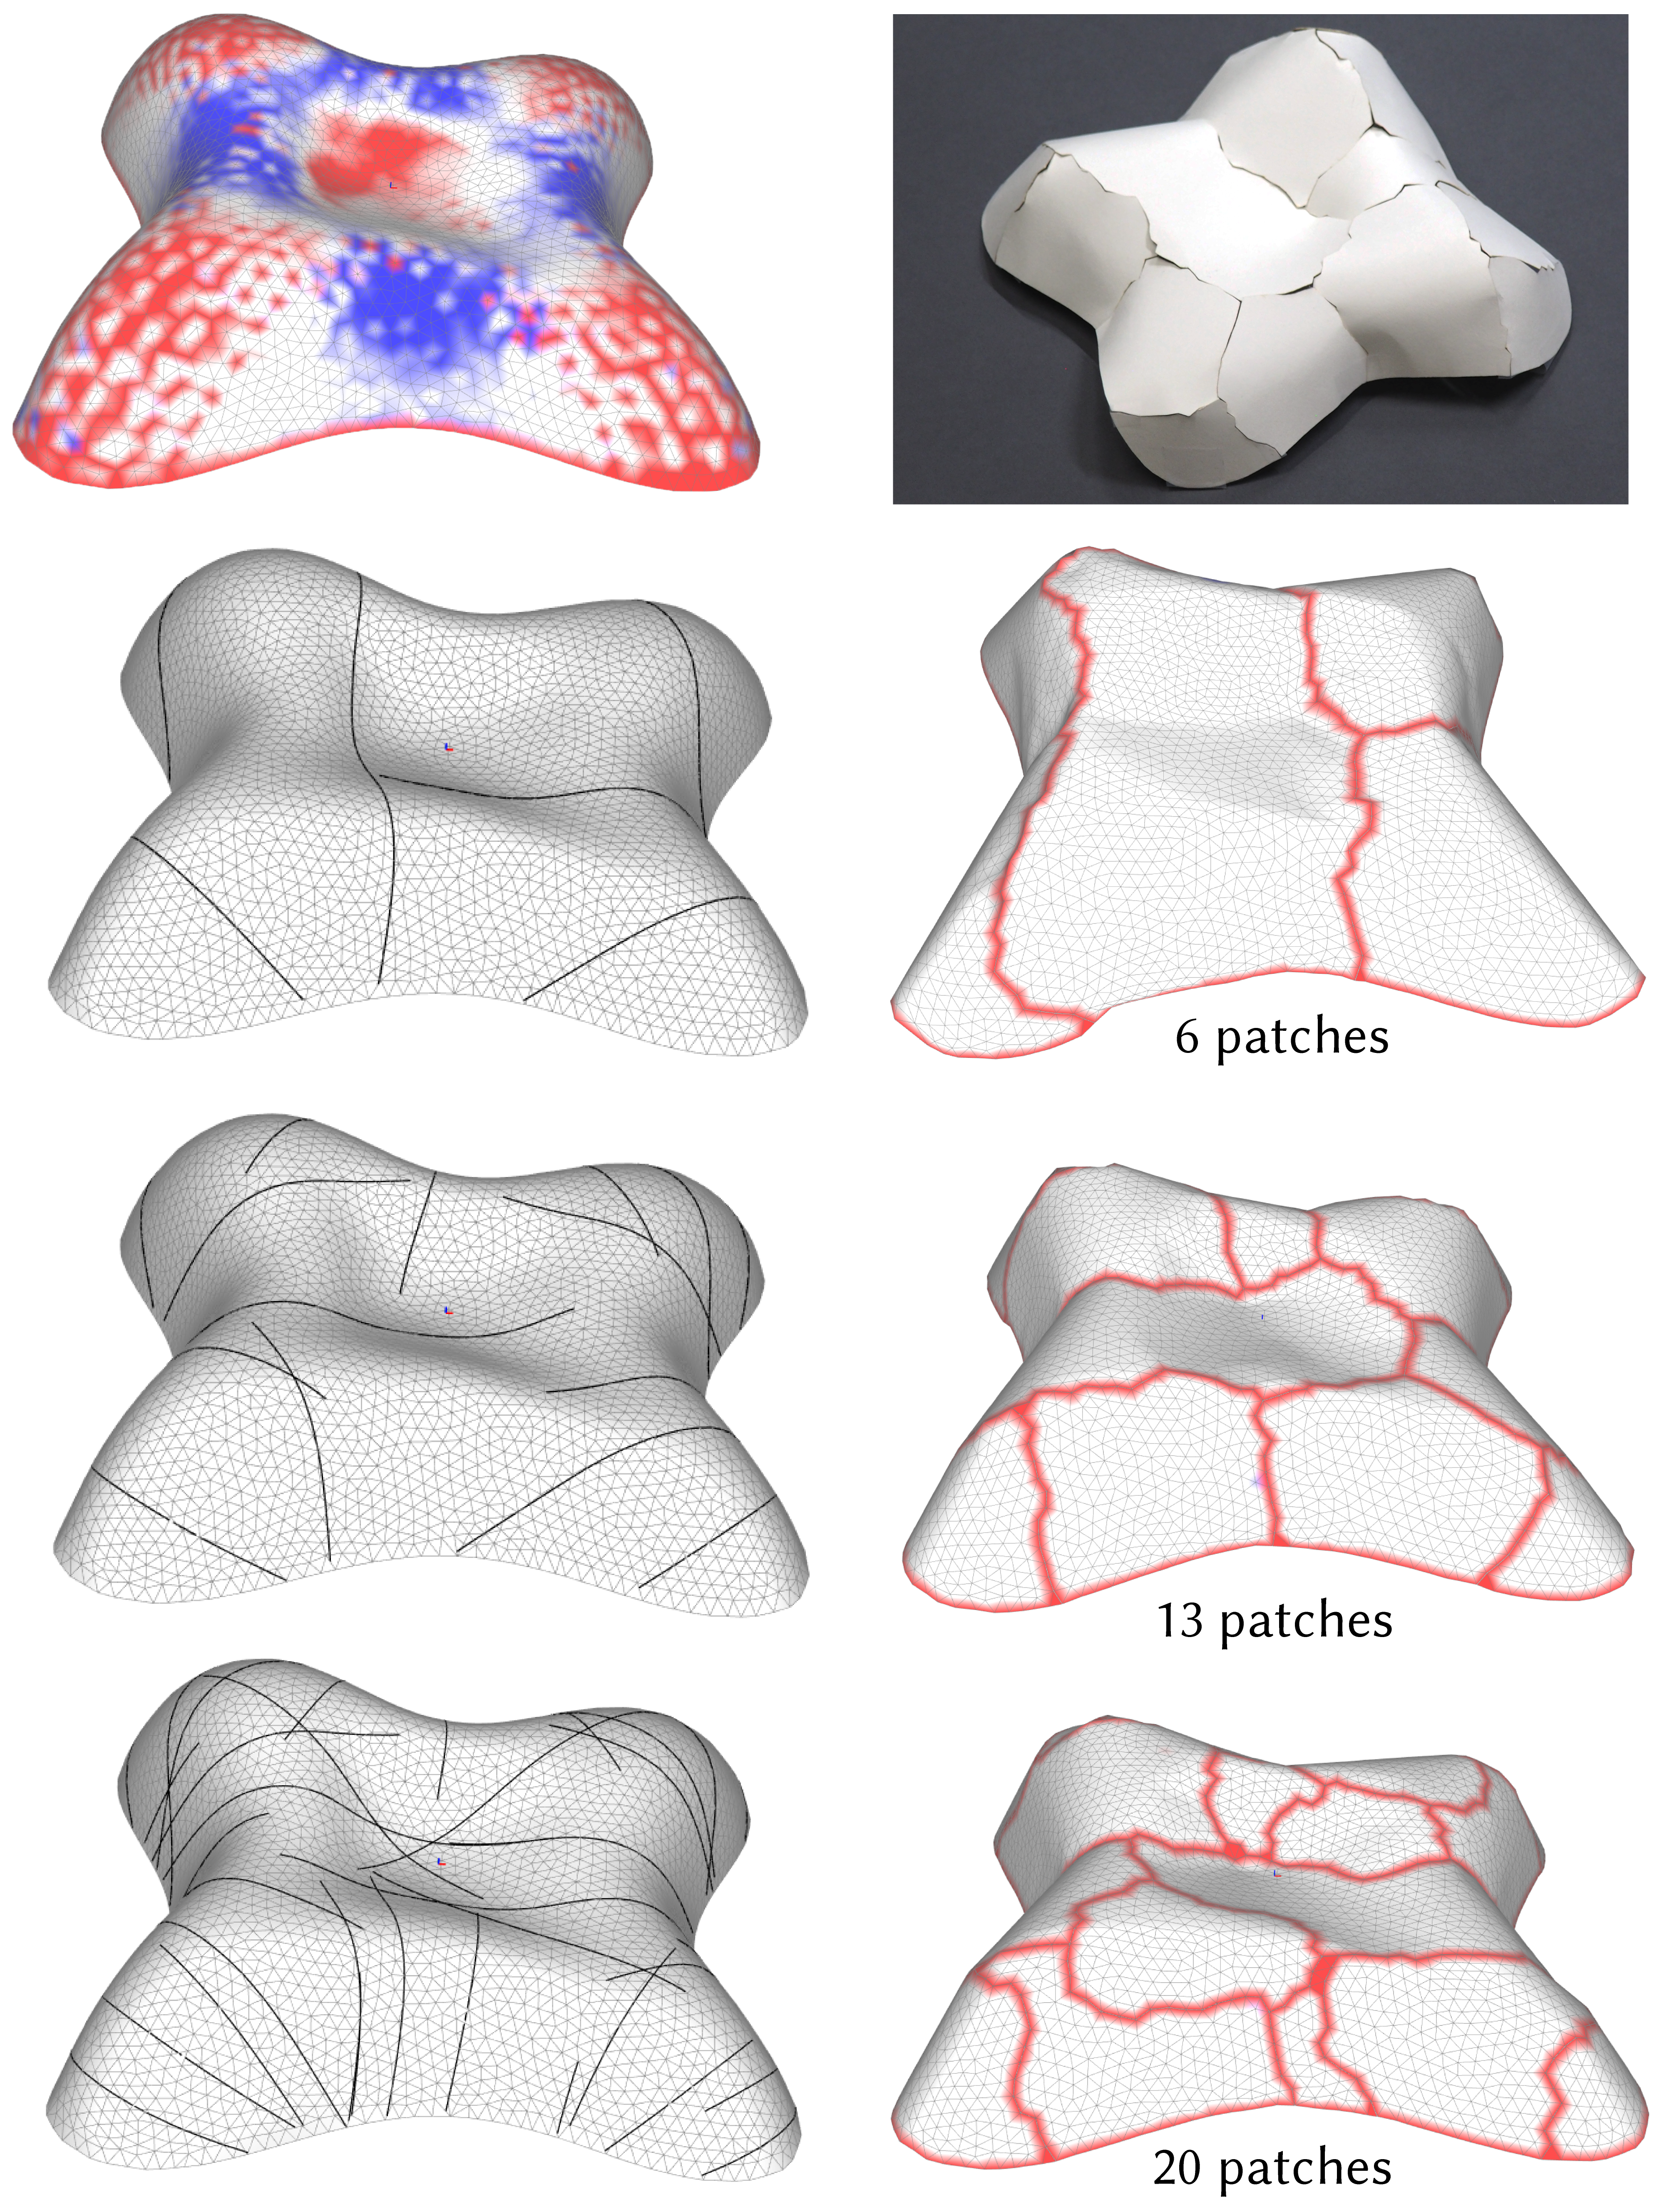
\includegraphics[width=\linewidth]{figures/FIG granularity 3x lilium grid-01.png}
% \caption{
% 	\AI{todo.}
% 	Our algorithm allows adapting the granularity of the resulting piecewise developable surface according to users' preferences. Naturally, fewer patches result in a higher approximation error. We show 3 versions of the same model, with 6, 13 and 20 patches and denote their Hausdorff distance $d_H$ and the total approximation error $\eps_\text{sum}$ as the sum of the per-vertex distance from $V_t$ to any point on the developable result. The metrics are relative to the shape's size, here bounding box diagonal is 28.8.\\
% 	\AI{- visual: remove mesh \& gauss from result, add error map, add used parameters of $ \lambda, \delta, \eps $.}\\
% 	\AI{- error values got lost! fix also in text}
% 	% \AI{add color scale, re-arrange image}
% 	\label{fig:granularity}}
% \end{figure}

% The granularity of the developable result is defined by 3 parameters, which we already discussed in the previous sections: 
% \begin{enumerate}
% 	\item $\lambda$, the penalty in the smoothness term of our geodesics selection, as it defines the number of DOG patches to approximate,
% 	\item $\delta_{\text{distance}}$, which defines how much the DOG patch can stretch to cover a larger surface, and
% 	\item $\eps_{\text{max}}$, the maximum per-vertex approximation error that defines areas considered as being uncovered.
% \end{enumerate}

% \todo{! show sensitivity to parameters here.}

% % \paragraph{Balanced granularity.}
% By default, our algorithm aims to balance the approximation error and the number of patches. The biggest influencing factor is the geodesics selection in our initialization procedure, governed by $\lambda$. This defines how many DOG patches are fitted to the target shape. A lower value results in more patches and therefore in a higher granularity. Conversely, a higher smoothness value results in lower granularity. 
% Based on the user-defined smoothness value, we automatically adapt the value of $\delta_{\text{distance}}$, where a higher value allows for more stretch and more deviation from the target surface. We adapt $\delta_{\text{distance}}$ relative to the average edge length $\overline{e}$ of the target $\target$. We interpolate $\delta_{\text{distance}}$ between $ 4 \overline{e} $ for low granularity and $ 0.9 \overline{e} $ for high granularity, as we empirically found good approximation results within these bounds. 
% The approximation error $\eps_{\text{max}}$ is an absolute threshold independent of the mesh resolution. The default value in our implementation is $0.8$. 

% The initial number of selected geodesics might not be the resulting number of piecewise developables, as additional patches are added for uncovered areas. 
% To control the number of developable parts, users can disable the approximation error $\eps_\text{max}$ by setting it very high such that no uncovered areas are detected. 
% Conversely, setting $\eps_\text{max}$ allows users to create results with a user-defined maximum approximation error since uncovered areas will be approximated until all are covered.

% % \paragraph{Specifying the number of patches.}
% % To force the algorithm to stick to n parts, we can disable the hole patching and set the outlier threshold <high> to allow for stretching and thus coverage with few patches.

% % \paragraph{Specifying the approximation error.} 
% % Enforcing a maximum approximation error is trickier. Mainly, we need to select geodesics until we get an approximation error of <2 * max. Error>. this is because the ruled surfaces are not precise and the DOG patches typically fit way better. Of course, the coverage threshold is then set to <max. Error * 0.8 or so>. At the Result step, we select (by lowering the smoothness) until we found an assignment with the desired max. Error, disregarding the number of patches.


% % \paragraph{}

% In \figref{fig:granularity}, we note that the error values of the version with 13 and 20 patches are very similar, considering that they differ by 7 patches. This suggests a pareto-optimal front that governs the tradeoff between number of patches and approximation error. While it is outside the scope of this paper, we think that investigating how this might relate to the surface properties of a shape is an interesting opportunity for future work.


\end{document} 